\documentclass[10pt,a4paper]{article}
\usepackage[utf8]{inputenc}
\usepackage{amsmath}
\usepackage{gensymb}
\usepackage{amsfonts}
\usepackage{siunitx}
\usepackage[european]{circuitikz}
\usepackage{geometry}
\newgeometry{tmargin=2cm, bmargin=2cm, lmargin=2cm, rmargin=2cm}
\usepackage{amssymb}
\usepackage{polski}
\usepackage{graphicx}
\author{\textbf{T. Fąs}}
\title{\textbf{TERMISTOR JAKO TERMOMETR}}
\begin{document}
\maketitle

\begin{center}
\textbf{\subsection*{STRESZCZENIE}}
\end{center}
Celem doświadczenia była kalibracja termistora tak, aby układ o określonym oporze złożony z termistora oraz woltomierza mógł służyć jako termometr. Otrzymano liniową zależność temperatury od napięcia na termistorze postaci $t(U)=\hat{H} U+\hat{G}$, gdzie $\hat{H}=-7,196\pm0,069$ $^{\circ}$C/V, $\hat{G}=140,41\pm0,72$ $^{\circ}$C, a ocena kowariancji pomiędzy $\hat{H}$ i $\hat{G}$ wynosi $c_{HG}=-0,04987$ $^{\circ}$C$^2$/V.

\begin{center}
\textbf{\subsection*{WSTĘP}}
\end{center}
Termistor jest rezystorem o oporze wrażliwym na zmiany temperatury. Wraz ze wzrostem temperatury maleje opór termistora. Jego wrażliwość na zmiany temperatury czyni z niego potencjalny termometr o wysokiej dokładności. Dokładna zależność oporu $r$ termistora od temperatury $T$ dana jest wzorem:
\begin{equation}
r(T)=r_{\infty}\exp{\left(\dfrac{B}{T}\right)},
\end{equation}
gdzie $B$ oraz $r_{\infty}$ są stałymi charakteryzującymi dany termistor \cite{pf}, a temperatura wyrażona jest w skali Kelvina.  
Aby móc wykorzystać wrażliwość termistora na zmiany temperatury należy podłączyć go do obwodu w sposób przedstawiony na Rysunku 1. Symbolem $R$ oznaczono tu opornik, którego wartość dobrano tak, by napięcie na termistorze silnie zależało od jego temperatury. Poprzez symbol $E$ rozumiemy tu źródło SEM, a $V(T)$ to napięcie mierzone na termistorze. Tak skonstruowany obwód nazywa się dzielnikiem napięć.
\begin{figure}[h!]
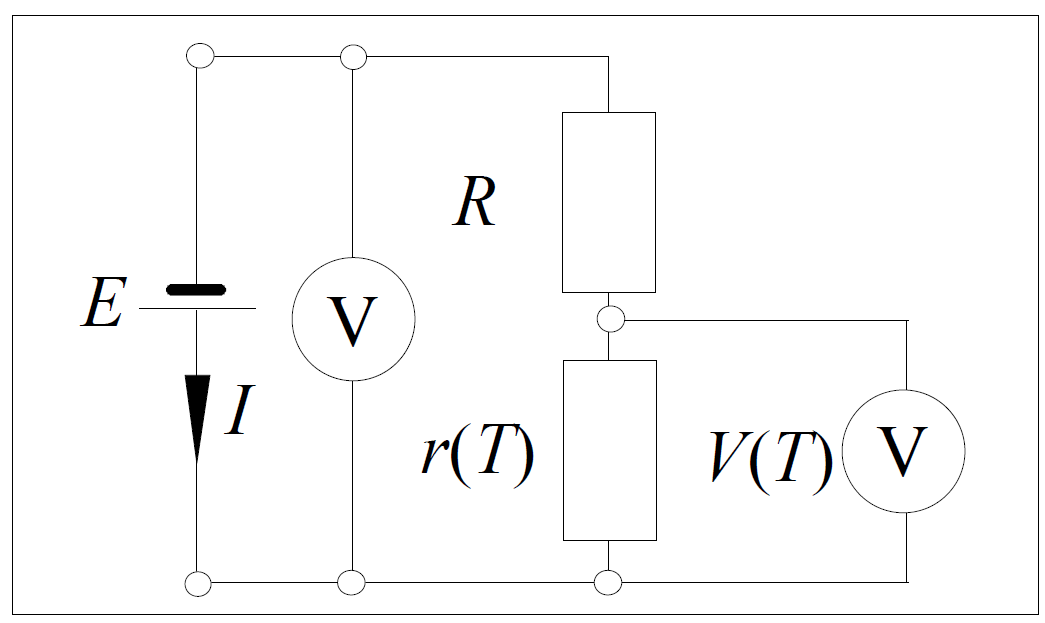
\includegraphics[width=8cm]{obwod} 
\centering
\caption{Schemat obwodu.}
\label{p1}
\end{figure}

Korzystają z prawa Kirchhoffa można znaleźć wzór opisujący zależność napięcia od temperatury, który przyjmuje następującą postać:
\begin{equation}
V(T)=\dfrac{r(T)}{R+r(T)}E
\end{equation}
Niewielkie zmiany temperatury wokół punktu $T_{0}$ mogą zostać wyznaczone z zadowalającą dokładnością korzystając z przybliżenia Równania (2) do postaci liniowej:
\begin{equation}
V(T)\approx h(T-T_{0})+V_{0},
\end{equation}
co po zamianie temperatury na skalę Celsjusza oraz zapisanie stałych w postaci jednej stałej $g$ sprowadza się do wzoru:
\begin{equation}
U(t)=ht+g.
\end{equation}
Zastosowano zamianę symbolu $V$ na $U$ aby odróżnić przybliżenie od dokładnej wartości.
Aby móc skonstruować termometr należy wyznaczyć wartości $B$ oraz $r_{\infty}$, które są potrzebne do wyznaczenia wartości $R$. Najdokładniejsze przybliżenie $U$ można uzyskać dla wartości $R$ obliczonej na podstawie punktu przegięcia funkcji $V(T)$. Dzięki takiemu założeniu można pozbyć się wyrazu kwadratowego w rozwinięciu Taylora, więc przybliżenie liniowe będzie charakteryzowało się większą dokładnością. Otrzymano następujący wzór pozwalający wyznaczyć wartość $R$:
\begin{equation}
R=\dfrac{B-2T}{B+2T}r_{\infty}\exp{\left(\dfrac{B}{T}\right)}
\end{equation}
 Następnie należy wyznaczyć wartości współczynników $h$ oraz $g$ z Równania (4). Ostatnim krokiem będzie odwrócenie zależności opisanej Równaniem (4) i wyznaczenie niepewności tak otrzymanej wartości temperatury.
\begin{center}
\textbf{\subsection*{UKŁAD DOŚWIADCZALNY}}
\end{center}
Układ doświadczalny składał się z termistora opatrzonego numerem 14, termometru o działce odczytu 0,1 $^{\circ}$C, którego wskazania traktowano jako dokładne oraz z miernika uniwersalnego Brymen 805 i miernika CHY 38. Niepewności pomiaru miernika Brymen obliczono na podstawie instrukcji dołączonej przez producenta \cite{b1}. Termistor oraz termometr były połączone ze sobą w taki sposób, aby wartości temperatury odczytywane na termometrze wzorcowym można było uznać za temperaturę termistora. Dodatkowo w dalszej części pomiarów wykorzystano płytkę drukowaną z miejscem na podłączenie oporników, zasilania oraz mierników. Po złożeniu układ był zgodny ze schematem przedstawionym na Rysunku 1. Wykorzystano go do zmierzenia zależności napięcia od temperatury dla wybranego opornika $R$. 

W pierwszej części pomiarów termistor podłączono do miernika Brymen w funkcji omomierza, a sam termistor zanurzono w wodzie o temperaturze początkowej około 80 $^{\circ}$C. Przez 30 min notowano wartości oporu dla danej temperatury. Zmierzono kilkadziesiąt wartości oporu i temperatury. Aby uczynić pomiar dokładniejszym zastąpiono gorącą wodę inną, schłodzoną do temperatury początkowej około 5 $^{\circ}$C. W tym przypadku również wykonywano pomiary przez 30 min. Jednak ze względu na powolny wzrost temperatury cieczy odnotowano jedynie kilkanaście pomiarów. Korzystając z paru punktów otrzymanych w tych pomiarach wyznaczono wstępne oceny parametrów $B$ oraz $r_{\infty}$, a stąd oszacowanie wartości $R$. Wybrano opornik, którego opór był najbliższy wartości $R$. Dla tak wybranego opornika skonstruowano obwód zgodnie ze schematem przedstawionym na Rysunku 1. Po raz kolejny wykonywano pomiary prze 30 minut. Napięcie na termistorze mierzono miernikiem Brymen, a temperaturę wzorcowym termometrem. Z kolei napięcie na źródle mierzono przy pomocy mirnika CHY. Pomiary miernikiem CHY miały na celu zbadanie stabilności napięcia wysyłanego przez źródło. 

\begin{center}
\textbf{\subsection*{WYNIKI POMIARÓW}}
\end{center}
Wyniki pomiarów oporu w zależności od temperatury przedstawiono w Tabeli 1.
\begin{center}
 \begin{table}[h!]
 \centering
 \caption{Wartości oporu i temperatury.}
 \begin{tabular}{|c|c||c|c||c|c|c|c|c|c|c|}
 \hline
Opór $r$ [k$\Omega$]&Temp. t [$^{\circ}$C]&Opór $r$ [k$\Omega$]&Temp. t [$^{\circ}$C]&Opór $r$ [k$\Omega$]&Temp. t [$^{\circ}$C]\\
\hline
40,3&77&64&62&89,1&52\\
\hline
41,2&75,8&65&61,5&91&51,5\\
\hline
42,1&75&65,9&61&92,5&51\\
\hline
43,3&74,5&66,6&60,5&94,1&50,5\\
\hline
44&74&60&57&95,9&50\\
\hline
45&73,2&69&59,5&551&5\\
\hline
45,5&72,9&70&59,1&543&5,2\\
\hline
47,2&71,5&70,7&58,9&537&5,5\\
\hline	
71,2&58,5&71,2&58,5&524&6\\
\hline
49,6&70&73&58&509&6,5\\
\hline
50,8&69,2&74,3&57,5&495&7,1\\
\hline
52,2&68,3&75,7&57&484&7,6\\
\hline
53,7&67,4&76,8&56,5&474&8,1\\
\hline
55,1&66,7&78,2&56&459&8,8\\
\hline
55,6&66,2&79,8&55,5&441&9,4\\
\hline
58,4&65&81&55&434&9,9\\
\hline
59,3&64,5&82,4&54,5&425&10,2\\
\hline
60,2&64&83,8&54&420&10,7\\
\hline
61,8&63,2&58&53,5&413&11,1\\
\hline
62,2&63&86,2&53&410&11,4\\
\hline
63,1&62,5&87,6&52,5&400&11,9\\
\hline

 \end{tabular}
 \end{table}
 \end{center}

Na podstawie danych zawartych w Tabeli 1 wstępnie oszacowano wartości $B\approx3535$ K oraz $r_{\infty}\approx1,66$ $\Omega$ jak i również założone, iż punkt przegięcia znajduje się w okolicach 65 $^{\circ}$C. Na tej podstawie, wykorzystując Równanie (5), oszacowano wartość $R\approx37,8$ k$\Omega$. Wybrano opornik o oporze $R_{o}=41,7$ k$\Omega$, którego wartość była najbliższa wartości otrzymanej teoretycznie. Wartość tego oporu zmierzono korzystając z miernika Brymen. 
Ten opornik, jak i termistor wraz z termometrem podłączono do obwodu zgodnie ze schematem przedstawionym na Rysunku 1. Przy pomocy miernika Brymen zmierzono wartości napięcia panującego na termistorze, jak i temperaturę odpowiadającą danemu napięciu. Dane zebrane w trakcie tych pomiarów zebrano w Tabeli 2.

\begin{center}
 \begin{table}[h!]
 \centering
 \caption{Wartości napięcia i temperatury.}
 \begin{tabular}{|c|c||c|c|c|c|c|c|c|c|c|}
 \hline
Temp. t [$^{\circ}$C]&Napięcie $U$ [V]&Temp. t [$^{\circ}$C]&Napięcie $U$ [V]\\
\hline
75,2&9,07&63,9&10,66\\
\hline
74&9,21&63,5&10,71\\
\hline
73,3&9,33&63&10,75\\
\hline
72,8&9,41&62,5&10,86\\
\hline
72,3&9,48&62&10,92\\
\hline
71,7&9,6&61,5&10,97\\
\hline
71&9,67&61&11,04\\
\hline
70,5&9,72&60,5&11,1\\
\hline
70&9,73&59,9&11,18\\
\hline
69,3&9,86&59,5&11,22\\
\hline
68,7&9,96&59&11,32\\
\hline
68&10,05&58,5&11,39\\
\hline
67,5&10,12&58&11,46\\
\hline
67,2&10,15&57,5&11,52\\
\hline
66,7&10,22&57&11,59\\
\hline
66,3&10,29&56,5&11,67\\
\hline
65,6&10,38&56&11,73\\
\hline
64,9&10,48&55,5&11,8\\
\hline
64,5&10,57&55&11,86\\
\hline


 \end{tabular}
 \end{table}
 \end{center}
W trakcie wykonywania pomiarów napięcie na źródle oscylowało pomiędzy wartością 18,05, a 18,06 V. Jako, że odchylenia pokrywają się z działką odczytu to można założyć, że przyłożone napięcie było stałe.

\begin{center}
\textbf{\subsection*{ANALIZA DANYCH}}
\end{center}
Dla danych zawartych w Tabeli 1 wykonano wykres zależności $r(t)$ przedstawiony na Rysunku 2.
\begin{figure}[h!]
\centering
\begin{minipage}{.5\textwidth}
  \centering
  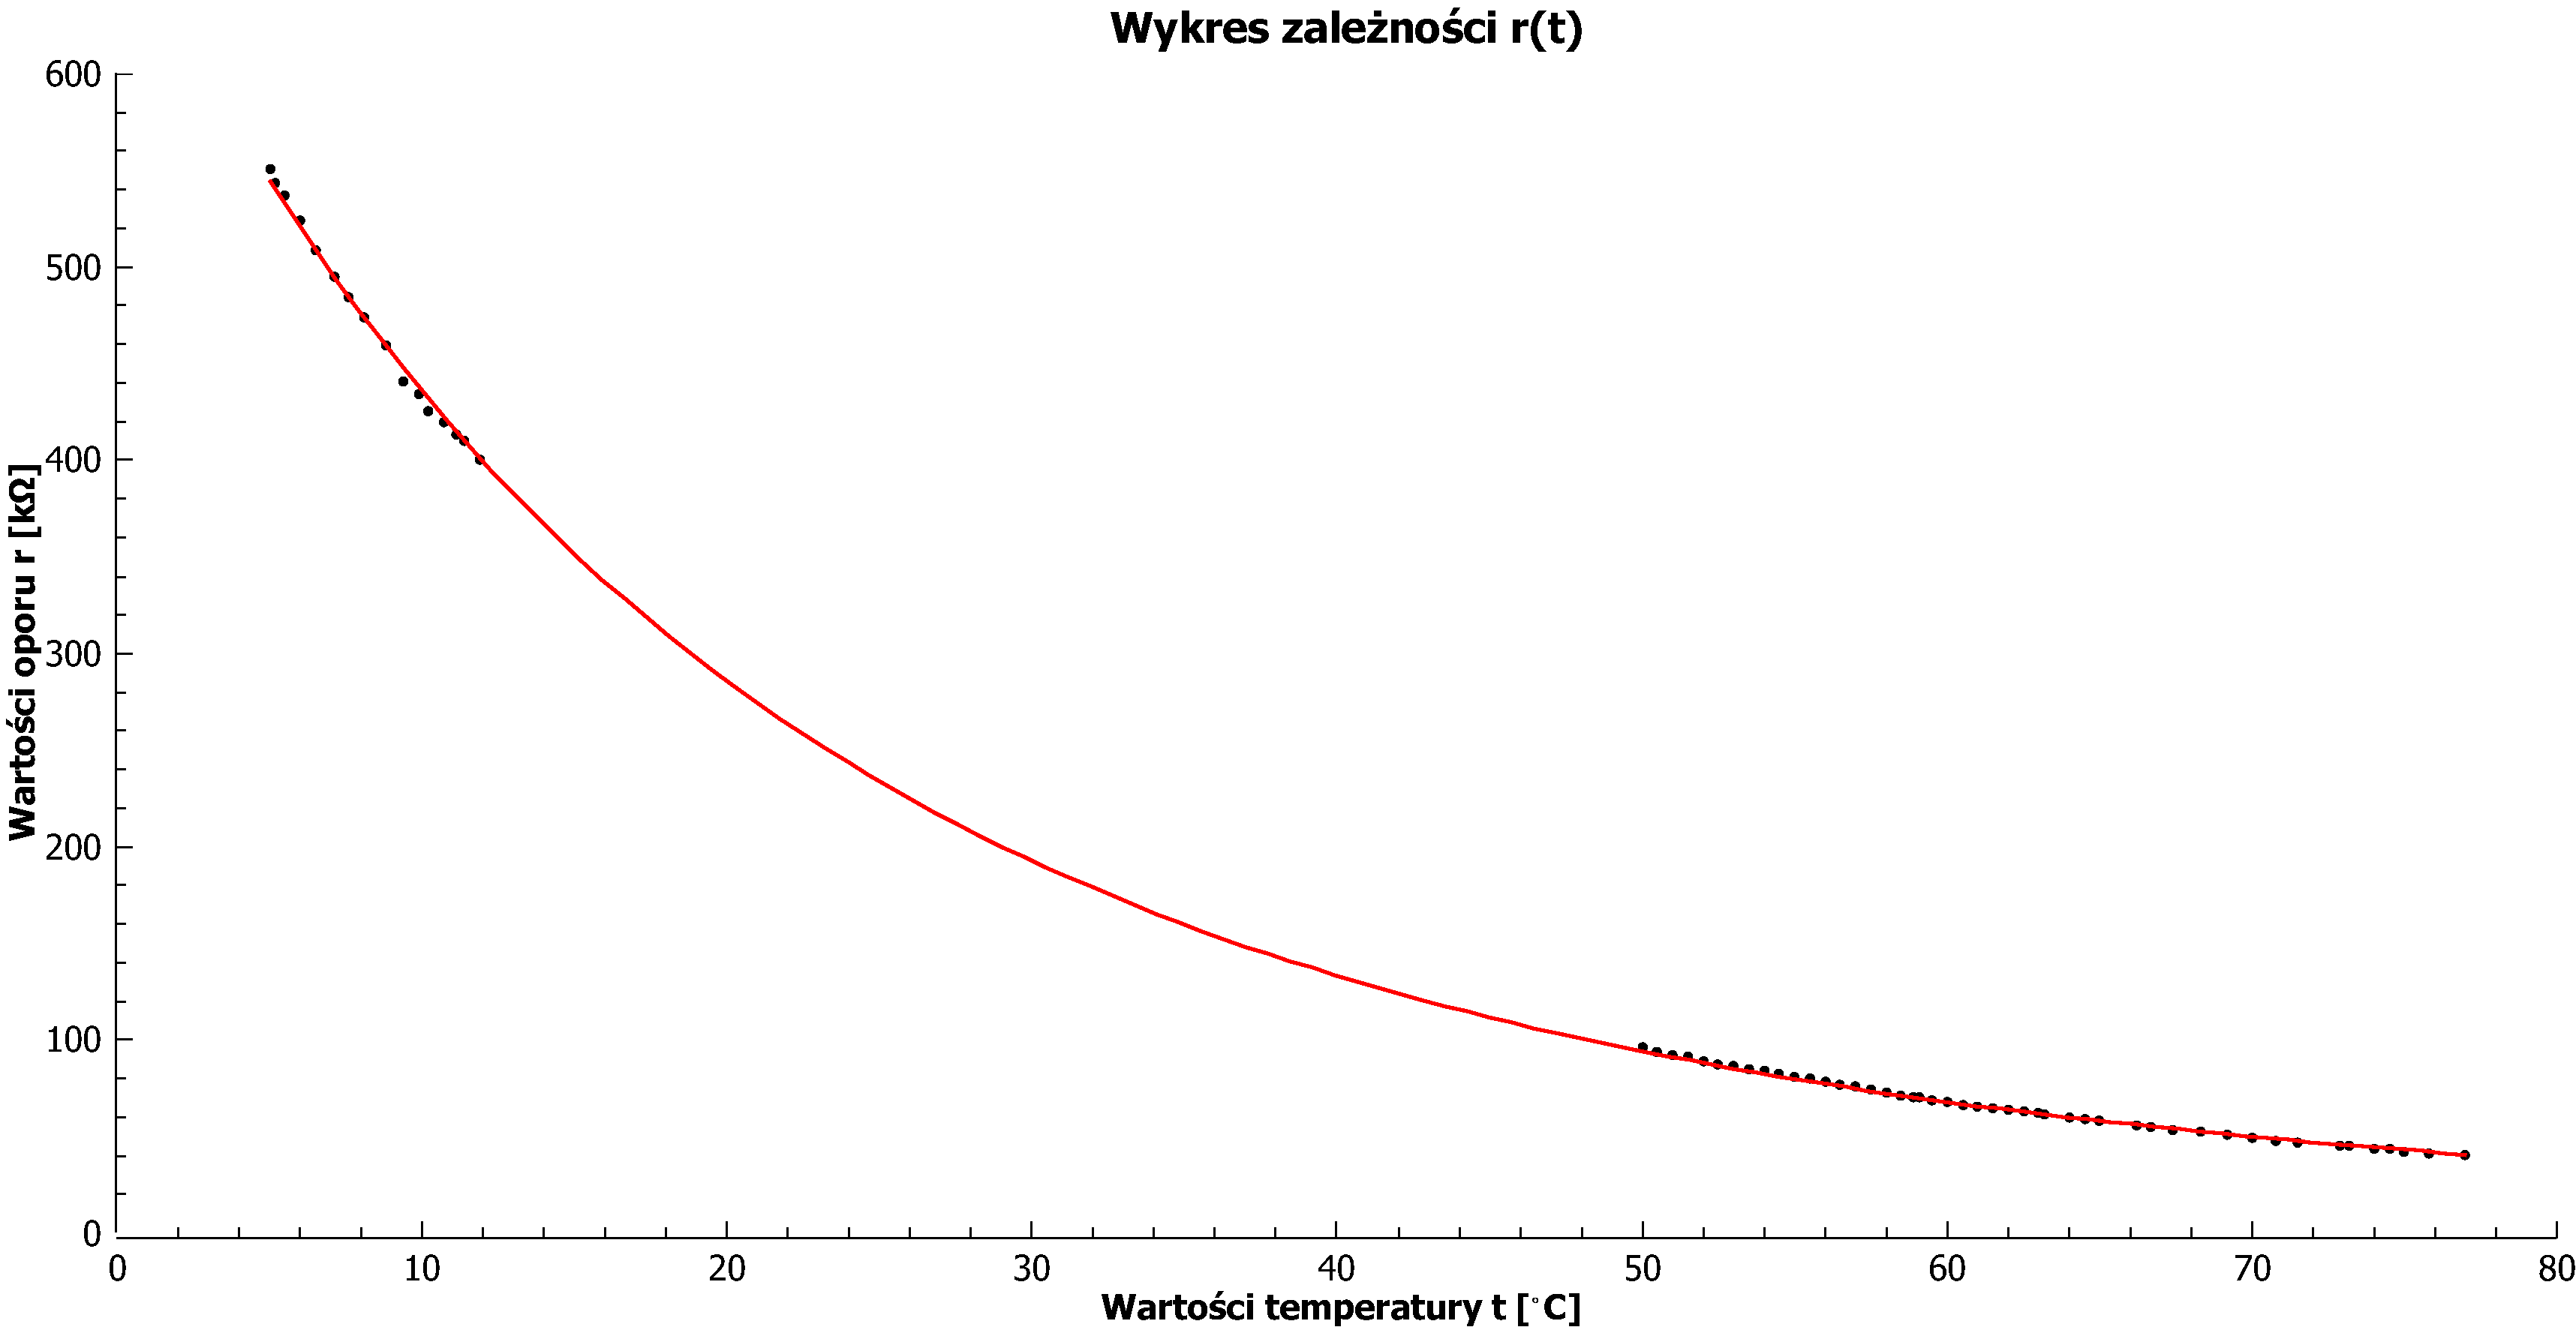
\includegraphics[width=10cm, height=6cm]{rys2.pdf} 
\caption{Wykres dla danych z Tabeli 1}
\end{minipage}%
\begin{minipage}{.5\textwidth}
  \centering
  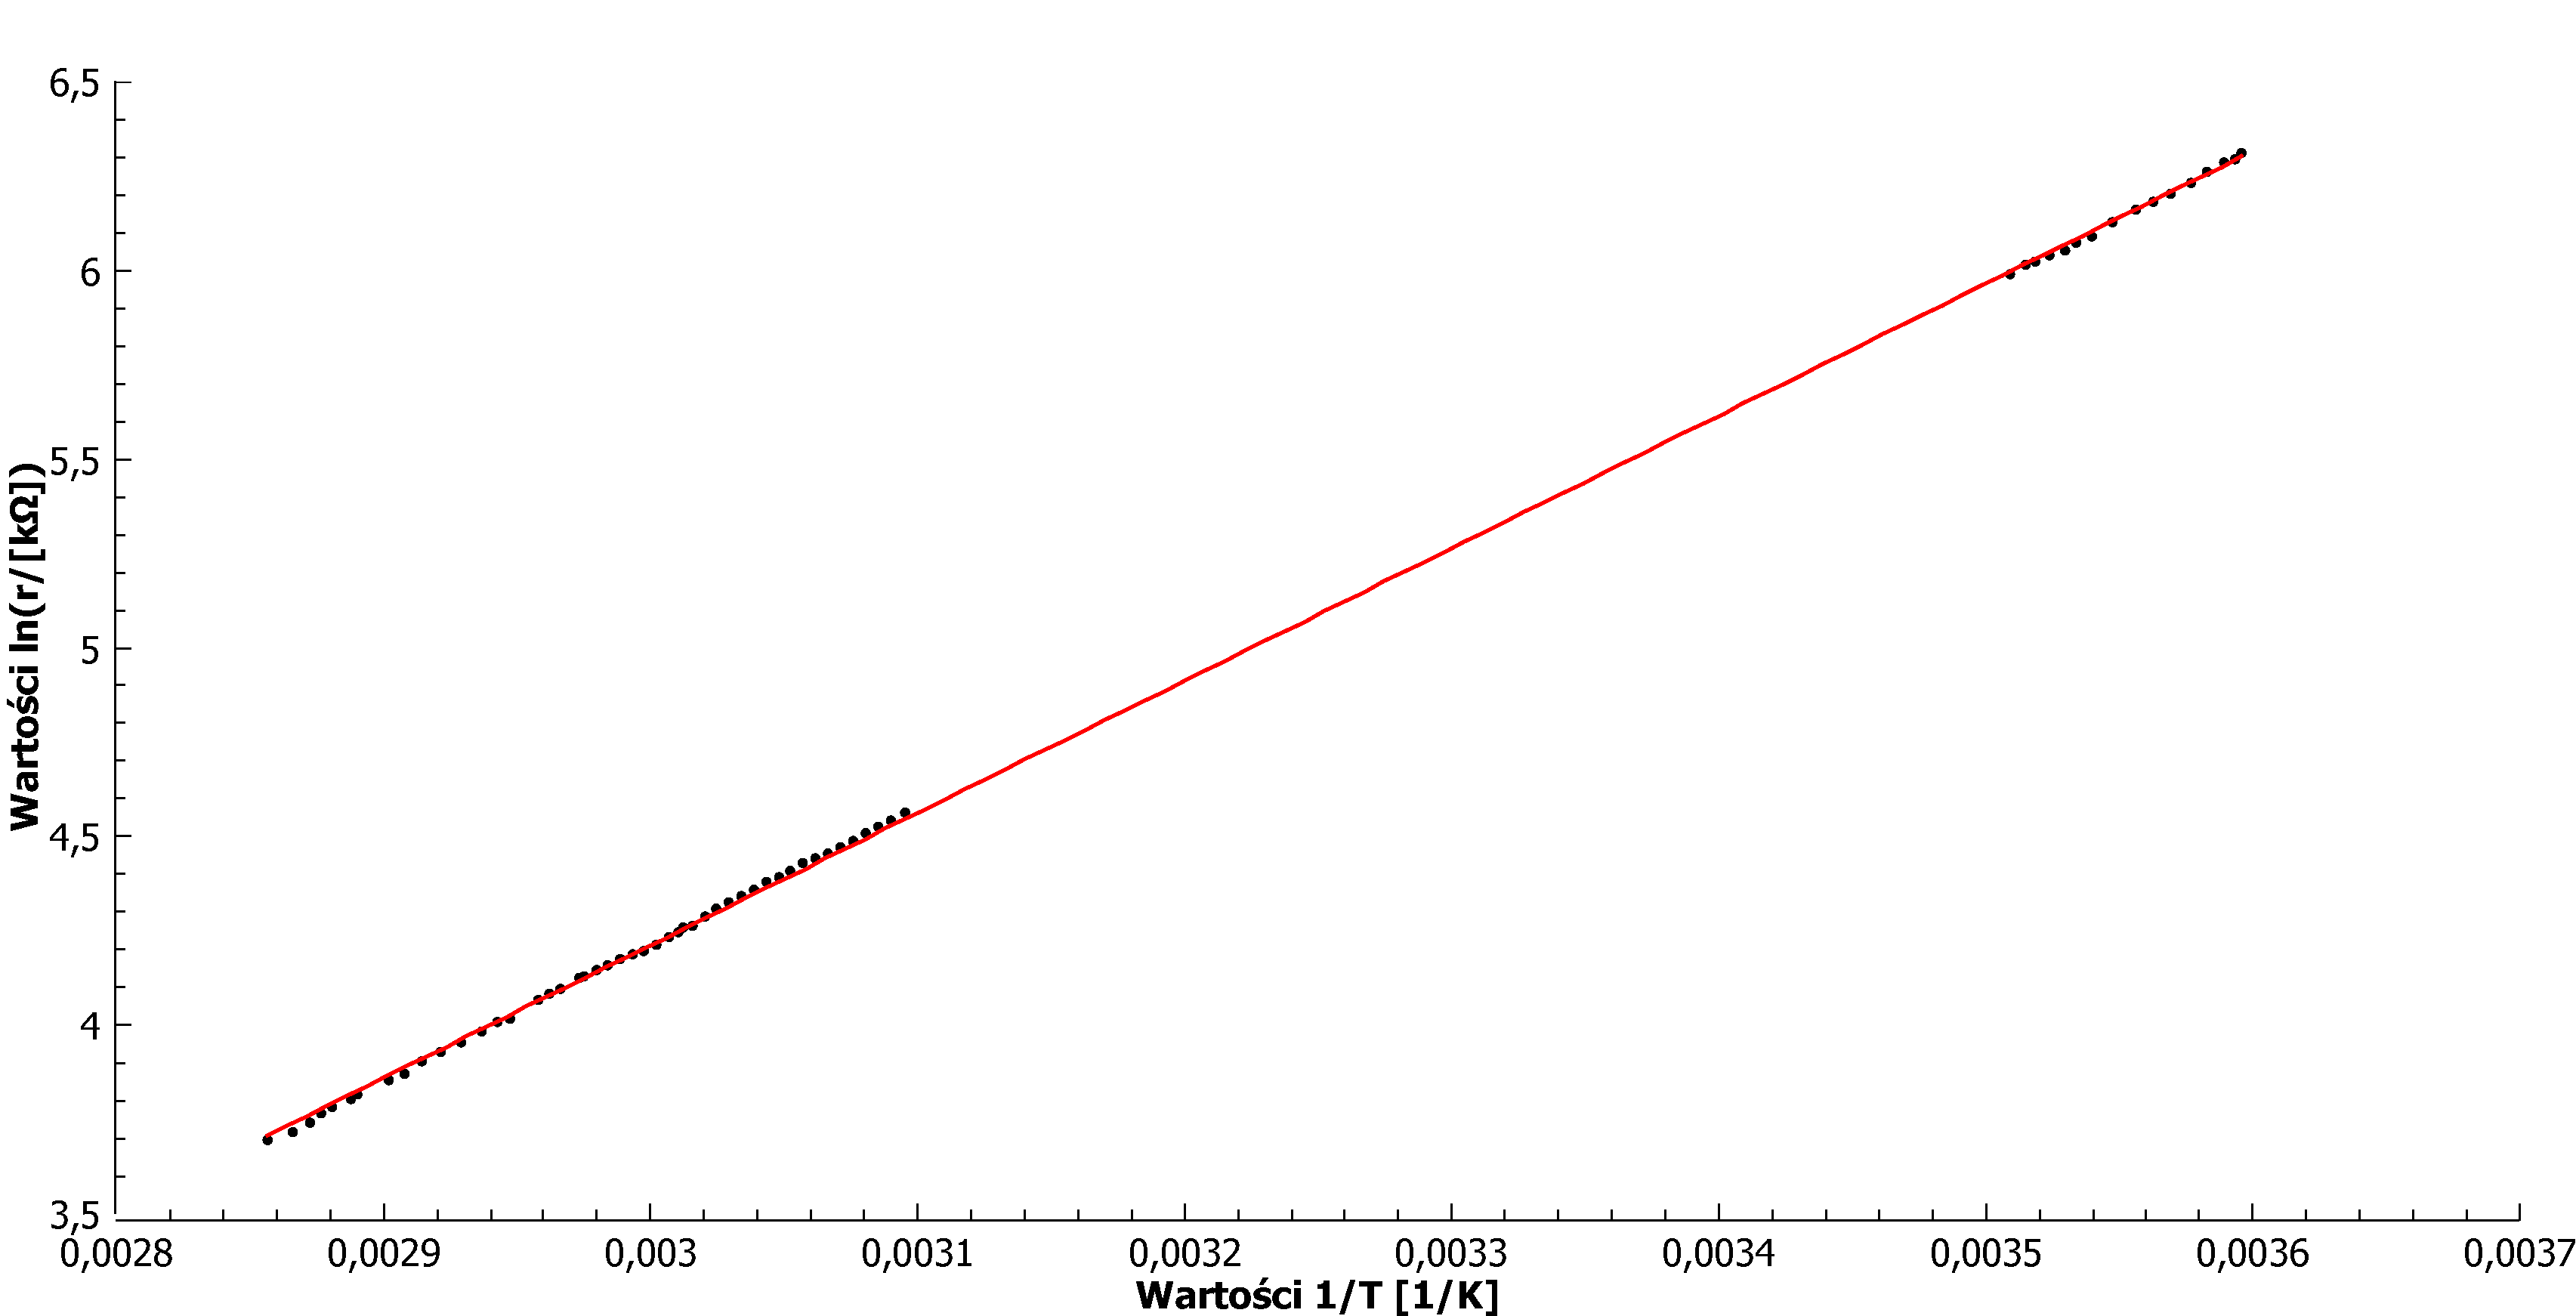
\includegraphics[width=10cm, height=6cm]{rys3.pdf} 
\caption{Wykres dla danych z Tabeli 3}
\end{minipage}
\end{figure}
Wyraźnie widać zależność eksponencjalną. Najlepszą metodą wyznaczenia współczynników $B$ oraz $r_{\infty}$ jest znalezienie krzywej najlepszego dopasowania. W tym celu należałoby zastosować metodę najmniejszych kwadratów. Jednak stosowanie jej do funkcji eksponencjalnej byłoby problematyczne, dlatego też zdecydowano się na sprowadzenie Równania (1) do postaci liniowej. Stosując obustronnie logarytm naturalny oraz podstawienia otrzymano zależność postaci:
\begin{equation}
\eta=\alpha x+\beta,
\end{equation}
gdzie $\eta=\log{\left(r/[\Omega]\right)}$, $\alpha=B$, $x=1/T$, a $\beta=\log{\left(r_{\infty}/[\Omega]\right)}$. W przypadku logarytmów zastosowano dzielenie przez jednostkę, aby uniknąć obliczania logarytmów z wartości mianowanych. Operacja tego typu byłaby pozbawiona sensu. Należy również wziąć pod uwagę fakt, że Równanie (1) jest słuszne tylko dla temperatury wyrażonej w skali Kelvina, dlatego też na potrzeby wyznaczania krzywej najlepszego dopasowania posługiwano się tą skalą, jak i stosowano wartości oporu w k$\Omega$. Korzystając z tych zależności stworzona Tabelę 3 oraz Rysunek 3 przedstawiający wykres zależności $\eta(x)$. 

\begin{center}
 \begin{table}[h!]
 \centering
 \caption{Wartości napięcia i temperatury.}
 \begin{tabular}{|c|c|c|c|c|c|c|c|c|c|c|}
 \hline
 $ln{(r/[k\Omega])}$ & 1/T [1/K]&$ln{(r/[k\Omega])}$ & 1/T [1/K]&$ln{(r/[k\Omega])}$ & 1/T [1/K]\\
 \hline
0,00286 & 3,69635 & 0,00298 & 4,15888 & 0,00308 & 4,48976 \\ \hline
0,00287 & 3,71844 & 0,00299 & 4,17439 & 0,00308 & 4,51086 \\ \hline
0,00287 & 3,74005 & 0,00299 & 4,18814 & 0,00309 & 4,52721 \\ \hline
0,00288 & 3,76815 & 0,00300 & 4,19870 & 0,00309 & 4,54436 \\ \hline
0,00288 & 3,78419 & 0,00300 & 4,21361 & 0,00310 & 4,56331 \\ \hline
0,00289 & 3,80666 & 0,00301 & 4,23411 & 0,00360 & 6,31173 \\ \hline
0,00289 & 3,81771 & 0,00301 & 4,24850 & 0,00359 & 6,29711 \\ \hline
0,00290 & 3,85439 & 0,00301 & 4,25845 & 0,00359 & 6,28600 \\ \hline
0,00291 & 3,87120 & 0,00302 & 4,26549 & 0,00358 & 6,26149 \\ \hline
0,00291 & 3,90399 & 0,00302 & 4,29046 & 0,00358 & 6,23245 \\ \hline
0,00292 & 3,92790 & 0,00302 & 4,30811 & 0,00357 & 6,20456 \\ \hline
0,00293 & 3,95508 & 0,00303 & 4,32678 & 0,00356 & 6,18208 \\ \hline
0,00294 & 3,98341 & 0,00303 & 4,34120 & 0,00356 & 6,16121 \\ \hline
0,00294 & 4,00915 & 0,00304 & 4,35927 & 0,00355 & 6,12905 \\ \hline
0,00295 & 4,01818 & 0,00304 & 4,37952 & 0,00354 & 6,08904 \\ \hline
0,00296 & 4,06732 & 0,00305 & 4,39445 & 0,00353 & 6,07304 \\ \hline
0,00296 & 4,08261 & 0,00305 & 4,41159 & 0,00353 & 6,05209 \\ \hline
0,00297 & 4,09767 & 0,00306 & 4,42843 & 0,00352 & 6,04025 \\ \hline
0,00297 & 4,12390 & 0,00306 & 4,44265 & 0,00352 & 6,02345 \\ \hline
0,00298 & 4,13035 & 0,00307 & 4,45667 & 0,00351 & 6,01616 \\ \hline
0,00298 & 4,14472 & 0,00307 & 4,47278 & 0,00351 & 5,99146 \\ \hline
 \end{tabular}
 \end{table}
 \end{center}

Widać niewielkie odchylenia od prostej, można więc przypuszczać, iż ocena parametrów prostej będzie dobrym przybliżeniem ich rzeczywistych wartości.
 

Metoda najlepszych kwadratów polega na minimalizacji wielkości podanej wzorem:
\begin{equation}
 R(\alpha,\beta)=\sum_{i=1}^n\left(\dfrac{\eta_i-\hat{\alpha}x-\hat{\beta}}{u_i}\right)^2 ,
\end{equation}
 gdzie $u_i$ są niepewnościami pomiarów oporu, $n$ jest liczbą pomiarów, a $\hat{\alpha}$ i $\hat{\beta}$ są poszukiwanymi, najlepszymi ocenami parametrów prostej \cite{tay1}. Aby stosować metodę najmniejszych kwadratów, należy wybrać zmienną niezależną, która będzie traktowana jako zanana dokładnie, tj. o zerowej niepewności. W naszym przypadku zmienną niezależną jest pomiar temperatury. 
 Niepewności $u_i$ pomiaru oporu obliczono korzystając z instrukcji dołączonej przez producenta. Dopuszczalny graniczny błąd wskazania na danym zakresie pomiarowym miernika wyznaczono na podstawie wzoru:
\begin{equation}
\Delta_{p}=pz+nc,
\end{equation}
gdzie poszczególne symbole oznaczają: p – wynik pomiaru, w – dokładność wskazanej wartości z wyrażona w procentach, nc – dokładność cyfrowa określana jako liczba n najmniej znaczących jednostek c odczytu. Wielkości w, n oraz c odczytano z instrukcji miernika. 
Ostateczna niepewność pojedynczego pomiaru wyrażona jest wzorem:
\begin{equation}
u_{i}=\dfrac{\Delta_{p}}{\sqrt{3}}.
\end{equation}
Stosując Równanie (8) oraz Równanie (9) stworzono Tabelę \ref{t1} oraz Tabelę \ref{t2}, w których zawarto wyniki pomiarów oporu z Tabeli 1 i Tabeli 2 wraz z ich niepewnościami. Tabele te umieszczono w Dodatku, ze względu na ich rozmiary. 




Znając niepewności można zacząć stosować metodę najmniejszych kwadratów. Minimalizacja wielkości wyrażonej Równaniem (7) prowadzi do następujących wzorów:
\begin{eqnarray*}
 \hat{\alpha}=\dfrac{1}{\Delta}\left(SS_{x\eta}-S_{x}S_{\eta}\right), \quad  u_{\alpha}^2=\dfrac{S}{\Delta}, \quad \hat{\beta}=\dfrac{1}{\Delta}\left(S_{\eta}S_{xx}-S_{x \eta}S_{x}\right), \quad u^2_{\beta}=\dfrac{\Delta}{S_{xx}},  \\
 S=\sum_{i=1}^{n}\dfrac{1}{u_{\eta i}^2}, \quad S_{x}=\sum_{i=1}^{n}\dfrac{x_{i}}{u_{\eta i}^2}, \quad S_{xx}=\sum_{i=1}^{n}\dfrac{x_{i}^2}{u_{\eta i}^2}, \quad S_{\eta}=\sum_{i=1}^{n}\dfrac{\eta_{i}}{u_{\eta i}^2}, \quad S_{x \eta}=\sum_{i=1}^{n}\dfrac{x_{i}\eta_{i}}{u_{\eta i}^2}, \quad \Delta=SS_{xx}-S_{x}^2.
 \end{eqnarray*}
 W tym przypadku $u_{\eta i}$ jest niepewnością $\eta_{i}$, którą wyznaczono korzystając z metody propagacji małych błędów. Ogólny wzór przenoszenia niepewności w tej metodzie jest następujący:
 \begin{equation}
 u_{f}^2=\sum_{i=1}^n \left( \dfrac{\partial f}{\partial x_{i}}u_{i}\right)^2+\sum_{i=1, i\neq j}^n \left( \dfrac{\partial f}{\partial x_{i}}\dfrac{\partial f}{\partial x_{j}}c_{ij}\right),
 \end{equation}
 gdzie wielkość $f$ zależy od wielkości $x_{i}$ o niepewnościach $u_{i}$ i o ocenach kowariancji $c_{ij}$ \cite{tay2}. W omawianym przypadku kowariancja pomiędzy $\eta$ a $r$ wynosi zero. Stosując Równanie (10) do zależności $\eta=\log{\left(r/[\Omega]\right)}$ otrzymano następujący wzór na określenie niepewności:
 \begin{equation}
 u_{\eta i}=\dfrac{u_{i}}{r}.
 \end{equation}
 Podstawiając wartości liczbowe otrzymano następujące wyniki:
 \begin{eqnarray*}
 S=1099434,03067, \quad S_{x}=3378,11487 \ \dfrac{1}{K}, \quad S_{xx}=10,42096 \ \dfrac{1}{K^2}, \\
  S_{\eta}=4914120,14112, \quad S_{x \eta}=15244,42898 \ \dfrac{1}{K}, \quad \Delta=45502,23581 \ \dfrac{1}{K^2}.
 \end{eqnarray*}
 Szczegółowe obliczenia, które doprowadziły do tych wyników znajdują się w Tabeli \ref{t3}, Tabeli \ref{t4}, Tabeli \ref{t5} i Tabeli \ref{t6}, które to są umieszczone w Dodatku.
 
Wykorzystując zależności $\hat{\alpha}=\hat{B}$, $x=1/T$, $\hat{\beta}=\log{\left(r_{\infty}/[\Omega]\right)}$ oraz stosując dane z Tabeli 1, Tabeli 2, Tabeli \ref{t1} i Tabeli \ref{t2} uzyskano oceny parametrów: $B=\hat{\alpha}=3511,5\pm4,9$ K, $\hat{\beta}=-6,320\pm0,015 \quad \Rightarrow \quad r_{\infty}=1,800\pm0,027$ $\Omega$. 
Niepewność $r_{\infty}$ otrzymano stosując Równanie (10) i otrzymując $u_{r}=\exp{(\beta)}u_{\beta}$.
Aby ocenić charakter zależności pomiędzy wielkościami $\hat{\alpha}$ oraz $\hat{\beta}$ należy wyznaczyć ocenę ich kowariancji $c_{\alpha \beta}$ oraz współczynnik korelacji $\rho_{\alpha \beta}$. Dla tych konkretnych wielkości wyrażają się one wzorami:
\begin{eqnarray}
 c_{\alpha \beta}=\dfrac{-S_{x}}{\Delta} \quad \cite{tay2}, \\
 \rho_{\alpha \beta}=\dfrac{c_{\alpha \beta}}{u_{\alpha} u_{\beta}} \quad \cite{tay3}.
 \end{eqnarray}
Podstawiając dane liczbowe otrzymano wartości $c_{\alpha \beta}=-0,07424$ K oraz $\rho_{\alpha \beta}=-0,99801$. Otrzymanie wartości $\rho$ bliskiej -1 świadczy o odwrotnej proporcjonalności porównywanych wielkości, tj wraz ze wzrostem $x$ maleje $\eta$. Aby przenieść ocenę kowariancji na wartości $B$ oraz $r_{\infty}$ należy zastosować wzór:
\begin{equation}
c_{Br}=\sum_{i=1}^n \dfrac{\partial B}{\partial x_{i}}\dfrac{\partial r}{\partial x_{j}}u_{i}+\sum_{i=1,i\neq j}^n \dfrac{\partial B}{\partial x_{i}}\dfrac{\partial r}{\partial x_{j}}c_{\alpha \beta} \quad \cite{tay2},
\end{equation}
który zwraca wartość $c_{Br}=exp{\beta}c_{\alpha \beta}=-0,00013$ K$\Omega$, a ocena korelacji $p_{Br}$ jest taka sama jak $\rho_{\alpha \beta}$, gdyż dodatkowy wyraz przy niepewności $r$ zredukuje się z analogicznym wyrazem w wartości $c_{Br}$. 

Znając dokładne wartości $B$ oraz $r_{\infty}$ można wyznaczyć dokładny opór dzielnika napięć, którego wartość wyraża się Równaniem (5). Podstawiając dane otrzymano wartość $R=39,49772$ k$\Omega$. Dodatkowo odwracając zależność z Równania (1) można wyznaczyć temperaturę, dla której byłby destynowany opornik użyty w pomiarach, którego opór wynosił $R_{p}=41,7$ k$\Omega$. Otrzymana wartość temperatury wynosi $t_{p}=76,25473$ $^{\circ}$C. Pomimo tego, że użyty opornik ostatecznie cechował się opornością bliższą tej oczekiwanej, niż pierwotnie sądzono, to nie pozwoliło to uniknąć rozbieżności w wartości temperatury punktu przegięcia. 

W dalszej części analizy danych zajęto się wyznaczaniem parametrów prostej opisanej Równaniem (4) na podstawie danych z Tabeli 2. Rysunek 4 przedstawia wykres zależności napięcia $U$ od temperatury $t$. Do wyznaczenia parametrów krzywej po raz kolejny zastosowano wykorzystano metodę najmniejszych kwadratów. Niepewności napięcia wyznaczono korzystając z Równania (8) oraz z instrukcji miernika. Otrzymane wzory służące do wyznaczenie najlepszych ocen parametrów prostej są analogiczne do wzorów wykorzystanych w poprzedniej analizie. Wartości napięć i ich niepewności przedstawia Tabela 4. 

\begin{figure}[h!]
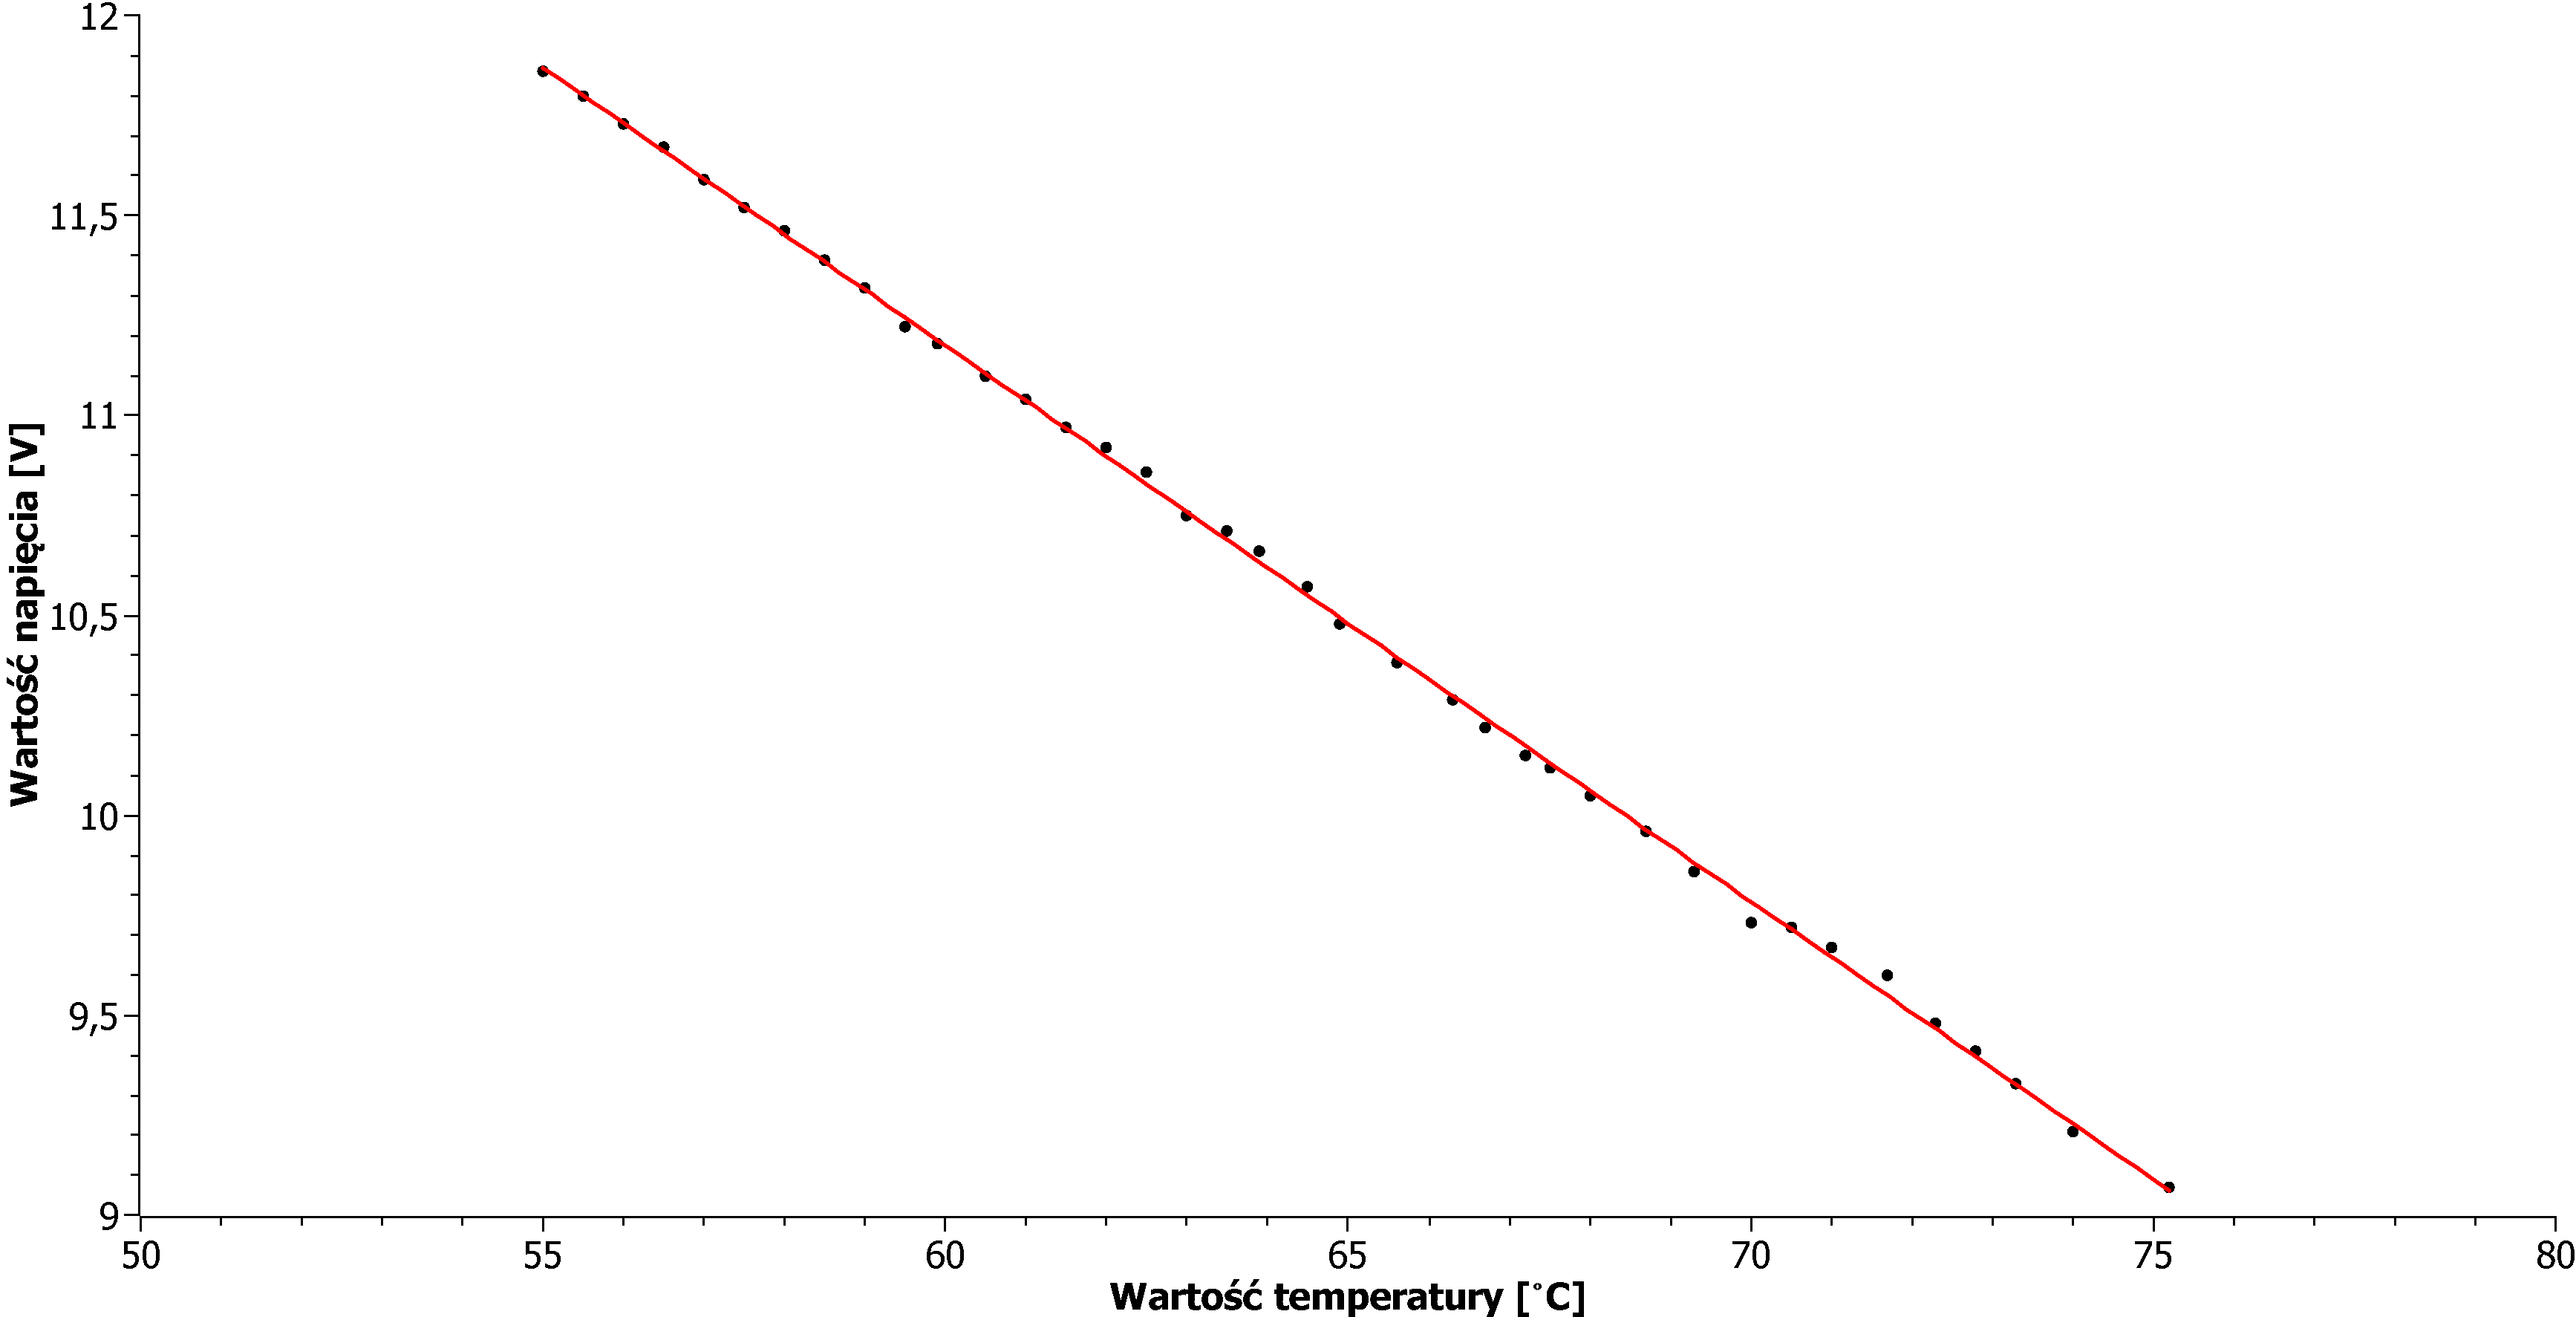
\includegraphics[width=10cm]{rys4.pdf} 
\centering
\caption{Wykres zależności $U(t)$}
\end{figure}

\begin{center}
 \begin{table}[h!]
 \centering
 \caption{Wartości napięcia oraz jego niepewności}
 \begin{tabular}{|c|c|c|c|c|c|c|c|c|c|c|c|c|c|c|c|c|c|c|c|c|c|}
 \hline
Napięcie $U$ [V]&Wartość w& Wartość nc&Wartość $\Delta_{p}$ [V]& $u_{i}$ [V]\\ 
\hline
9,07000  & 0,00500 & 0,03000 & 0,07535 & 0,04350 \\ \hline
9,21000  & 0,00500 & 0,03000 & 0,07605 & 0,04391 \\ \hline
9,33000  & 0,00500 & 0,03000 & 0,07665 & 0,04425 \\ \hline
9,41000  & 0,00500 & 0,03000 & 0,07705 & 0,04448 \\ \hline
9,48000  & 0,00500 & 0,03000 & 0,07740 & 0,04469 \\ \hline
9,60000  & 0,00500 & 0,03000 & 0,07800 & 0,04503 \\ \hline
9,67000  & 0,00500 & 0,03000 & 0,07835 & 0,04524 \\ \hline
9,72000  & 0,00500 & 0,03000 & 0,07860 & 0,04538 \\ \hline
9,73000  & 0,00500 & 0,03000 & 0,07865 & 0,04541 \\ \hline
9,86000  & 0,00500 & 0,03000 & 0,07930 & 0,04578 \\ \hline
9,96000  & 0,00500 & 0,03000 & 0,07980 & 0,04607 \\ \hline
10,05000 & 0,00500 & 0,03000 & 0,08025 & 0,04633 \\ \hline
10,12000 & 0,00500 & 0,03000 & 0,08060 & 0,04653 \\ \hline
10,15000 & 0,00500 & 0,03000 & 0,08075 & 0,04662 \\ \hline
10,22000 & 0,00500 & 0,03000 & 0,08110 & 0,04682 \\ \hline
10,29000 & 0,00500 & 0,03000 & 0,08145 & 0,04703 \\ \hline
10,38000 & 0,00500 & 0,03000 & 0,08190 & 0,04728 \\ \hline
10,48000 & 0,00500 & 0,03000 & 0,08240 & 0,04757 \\ \hline
10,57000 & 0,00500 & 0,03000 & 0,08285 & 0,04783 \\ \hline
10,66000 & 0,00500 & 0,03000 & 0,08330 & 0,04809 \\ \hline
10,71000 & 0,00500 & 0,03000 & 0,08355 & 0,04824 \\ \hline
10,75000 & 0,00500 & 0,03000 & 0,08375 & 0,04835 \\ \hline
10,86000 & 0,00500 & 0,03000 & 0,08430 & 0,04867 \\ \hline
10,92000 & 0,00500 & 0,03000 & 0,08460 & 0,04884 \\ \hline
10,97000 & 0,00500 & 0,03000 & 0,08485 & 0,04899 \\ \hline
11,04000 & 0,00500 & 0,03000 & 0,08520 & 0,04919 \\ \hline
11,10000 & 0,00500 & 0,03000 & 0,08550 & 0,04936 \\ \hline
11,18000 & 0,00500 & 0,03000 & 0,08590 & 0,04959 \\ \hline
11,22000 & 0,00500 & 0,03000 & 0,08610 & 0,04971 \\ \hline
11,32000 & 0,00500 & 0,03000 & 0,08660 & 0,05000 \\ \hline
11,39000 & 0,00500 & 0,03000 & 0,08695 & 0,05020 \\ \hline
11,46000 & 0,00500 & 0,03000 & 0,08730 & 0,05040 \\ \hline
11,52000 & 0,00500 & 0,03000 & 0,08760 & 0,05058 \\ \hline
11,59000 & 0,00500 & 0,03000 & 0,08795 & 0,05078 \\ \hline
11,67000 & 0,00500 & 0,03000 & 0,08835 & 0,05101 \\ \hline
11,73000 & 0,00500 & 0,03000 & 0,08865 & 0,05118 \\ \hline
11,80000 & 0,00500 & 0,03000 & 0,08900 & 0,05138 \\ \hline
11,86000 & 0,00500 & 0,03000 & 0,08930 & 0,05156 \\ \hline
 \end{tabular}
 \end{table}
 \end{center}
 
Tabela 5 prezentuje wartości składników sum występujących w metodzie najmniejszych kwadratów. 

\begin{center}
 \begin{table}[h!]
 \centering
 \caption{Wartości pośrednie}
 \begin{tabular}{|c|c|c|c|c|c|c|c|c|c|c|c|c|c|c|c|c|c|c|c|c|c|}
\hline
$1/u_{i}$ [1/V]     & $S_{i}$ [1/V$^2$]  & $S_{t}$ [$^{\circ}$C/V$^2$] & $S_{U}$ [1/V]& $S_{tt}$ [$^{\circ}$C$^2$/V$^2$] & $S_{Ut}$ [$^{\circ}$C/V]\\ \hline
22,98674 & 528,39018                & 39734,94187                 & 4792,49897                  & 2988067,62866 & 360395,92277 \\ \hline
22,77516 & 518,70785                & 38384,38067                 & 4777,29927                  & 2840444,16953 & 353520,14596 \\ \hline
22,59688 & 510,61896                & 37428,36973                 & 4764,07489                  & 2743499,50151 & 349206,68962 \\ \hline
22,47957 & 505,33103                & 36788,09912                 & 4755,16501                  & 2678173,61574 & 346176,01269 \\ \hline
22,37792 & 500,77119                & 36205,75687                 & 4747,31086                  & 2617676,22138 & 343230,57509 \\ \hline
22,20578 & 493,09665                & 35355,02959                 & 4733,72781                  & 2534955,62130 & 339408,28402 \\ \hline
22,10658 & 488,70103                & 34697,77303                 & 4725,73895                  & 2463541,88514 & 335527,46520 \\ \hline
22,03627 & 485,59719                & 34234,60171                 & 4720,00466                  & 2413539,42078 & 332760,32865 \\ \hline
22,02226 & 484,97997                & 33948,59778                 & 4718,85509                  & 2376401,84470 & 330319,85641 \\ \hline
21,84175 & 477,06206                & 33060,40083                 & 4703,83192                  & 2291085,77735 & 325975,55216 \\ \hline
21,70490 & 471,10257                & 32364,74645                 & 4692,18158                  & 2223458,08129 & 322352,87467 \\ \hline
21,58319 & 465,83399                & 31676,71121                 & 4681,63158                  & 2154016,36242 & 318350,94768 \\ \hline
21,48946 & 461,79707                & 31171,30208                 & 4673,38633                  & 2104062,89060 & 315453,57708 \\ \hline
21,44955 & 460,08301                & 30917,57805                 & 4669,84252                  & 2077661,24472 & 313813,41717 \\ \hline
21,35698 & 456,12045                & 30423,23417                 & 4661,55102                  & 2029229,71898 & 310925,45319 \\ \hline
21,26520 & 452,20887                & 29981,44813                 & 4653,22928                  & 1987770,01109 & 308509,10127 \\ \hline
21,14836 & 447,25319                & 29339,80956                 & 4642,48816                  & 1924691,50711 & 304547,22323 \\ \hline
21,02003 & 441,84183                & 28675,53492                 & 4630,50240                  & 1861042,21651 & 300519,60599 \\ \hline
20,90586 & 437,05514                & 28190,05634                 & 4619,67280                  & 1818258,63393 & 297968,89551 \\ \hline
20,79293 & 432,34581                & 27626,89710                 & 4608,80631                  & 1765358,72452 & 294502,72306 \\ \hline
20,73071 & 429,76233                & 27289,90800                 & 4602,75456                  & 1732909,15791 & 292274,91467 \\ \hline
20,68120 & 427,71219                & 26945,86768                 & 4597,90599                  & 1697589,66362 & 289668,07752 \\ \hline
20,54627 & 422,14933                & 26384,33319                 & 4584,54174                  & 1649020,82463 & 286533,85849 \\ \hline
20,47341 & 419,16067                & 25987,96171                 & 4577,23455                  & 1611253,62574 & 283788,54182 \\ \hline
20,41309 & 416,69430                & 25626,69955                 & 4571,13649                  & 1576042,02223 & 281124,89405 \\ \hline
20,32923 & 413,27779                & 25209,94512                 & 4562,58679                  & 1537806,65212 & 278317,79409 \\ \hline
20,25790 & 410,38268                & 24828,15225                 & 4555,24777                  & 1502103,21124 & 275592,49000 \\ \hline
20,16357 & 406,56962                & 24353,52042                 & 4545,44839                  & 1458775,87307 & 272272,35828 \\ \hline
20,11673 & 404,68299                & 24078,63800                 & 4540,54317                  & 1432678,96094 & 270162,31835 \\ \hline
20,00059 & 400,02347                & 23601,38461                 & 4528,26566                  & 1392481,69226 & 267167,67384 \\ \hline
19,92008 & 396,80952                & 23213,35687                 & 4519,66042                  & 1357981,37707 & 264400,13478 \\ \hline
19,84022 & 393,63415                & 22830,78062                 & 4511,04734                  & 1324185,27572 & 261640,74586 \\ \hline
19,77227 & 390,94264                & 22479,20185                 & 4503,65922                  & 1292554,10646 & 258960,40533 \\ \hline
19,69359 & 387,83729                & 22106,72571                 & 4495,03423                  & 1260083,36563 & 256216,95101 \\ \hline
19,60442 & 384,33342                & 21714,83806                 & 4485,17098                  & 1226888,35018 & 253412,16012 \\ \hline
19,53808 & 381,73658                & 21377,24831                 & 4477,77005                  & 1197125,90531 & 250755,12267 \\ \hline
19,46125 & 378,74006                & 21020,07322                 & 4469,13269                  & 1166614,06388 & 248036,86403 \\ \hline
19,39587 & 376,19961                & 20690,97836                 & 4461,72733                  & 1138003,80965 & 245395,00332 \\ \hline
\end{tabular}
 \end{table}
 \end{center}

Na podstawie danych z Tabeli 5 wyznaczono następujące wartości sum:
\begin{eqnarray*}
 S=16759,54666 \ \dfrac{1}{V^2}, \quad S_{t}=1089944,88273 \ \dfrac{^{\circ}C}{V^2}, \quad S_{tt}=71447033,01494 \ \dfrac{^{\circ}C^2}{V^2}, \\
  S_{U}=175560,66677 \ \dfrac{1}{V}
, \quad S_{Ut}=11339184,95965 \ \dfrac{^{\circ}C}{V}, \quad \Delta=9440036389,05640 \ \dfrac{^{\circ}C^2}{V^4}.
 \end{eqnarray*}
Obliczone parametry prostej wraz z niepewnościami wynoszą: $h=-0,1390\pm0,0013$ V/$^{\circ}$C i $g=19,513\pm0,087$ V. Na podstawie Równania (12) oraz Równania (13) obliczono ocenę kowariancji jak i ocenę korelacji pomiędzy $h$ i $g$. Otrzymano: $c_{hg}=-0,00012$ V$^2$/$^{\circ}$C i $\rho_{hg}=-0,99605$. Po raz kolejny ocena korelacji wskazuje na silnie skorelowaną zależność odwrotnie proporcjonalną. Wartość ta jest zgodna z oczekiwaniami.  Na potrzeby analizy danych obliczono również reszty napięć $\epsilon_{i}$, czyli różnice pomiędzy wartością zmierzoną $U_{i}$, a wartością teoretyczną obliczoną dla danej temperatury tj. $ht_{i}+g$. Wartości tych reszt są zaprezentowane w Tabeli 6, a ich wykres znajduje się na Rysunku 5.

\begin{center}
 \begin{table}[h!]
 \centering
 \caption{Wartości reszt}
 \begin{tabular}{|c|c|c|c|c|c|c|c|c|c|c|c|c|c|c|c|c|c|c|c|c|c|}
\hline
 Temperatura t [$^{\circ}$C]&75,2     & 74       & 73,3     & 72,8     & 72,3     & 71,7     & 71       \\ \hline
Reszta [V]&0,00743  & -0,01933 & 0,00340  & 0,01391  & 0,01443  & 0,05105  & 0,02377  \\ \hline
Temperatura t [$^{\circ}$C]&70,5     & 70       & 69,3     & 68,7     & 68       & 67,5     & 67,2     \\ \hline
Reszta [V]&0,00429  & -0,05519 & -0,02247 & -0,00585 & -0,01313 & -0,01261 & -0,02430 \\ \hline
Temperatura t [$^{\circ}$C]&66,7     & 66,3     & 65,6     & 64,9     & 64,5     & 63,9     & 63,5     \\ \hline
Reszta [V]&-0,02378 & -0,00937 & -0,01665 & -0,01392 & 0,02049  & 0,02711  & 0,02152  \\ \hline
Temperatura t [$^{\circ}$C]&63       & 62,5     & 62       & 61,5     & 61       & 60,5     & 59,9     \\ \hline
Reszta [V]&-0,00796 & 0,03256  & 0,02307  & 0,00359  & 0,00411  & -0,00538 & -0,00876 \\ \hline
Temperatura t [$^{\circ}$C]&59,5     & 59       & 58,5     & 58       & 57,5     & 57       & 56,5     \\ \hline
Reszta [V]&-0,02434 & 0,00617  & 0,00669  & 0,00721  & -0,00228 & -0,00176 & 0,00876  \\ \hline
Temperatura t [$^{\circ}$C]&56       &          &          & 55,5     &          &          & 55       \\ \hline
Reszta [V]&-0,00073 &          &          & -0,00021 &          &          & -0,00969 \\ \hline
\end{tabular}
 \end{table}
 \end{center}

\begin{figure}[h!]
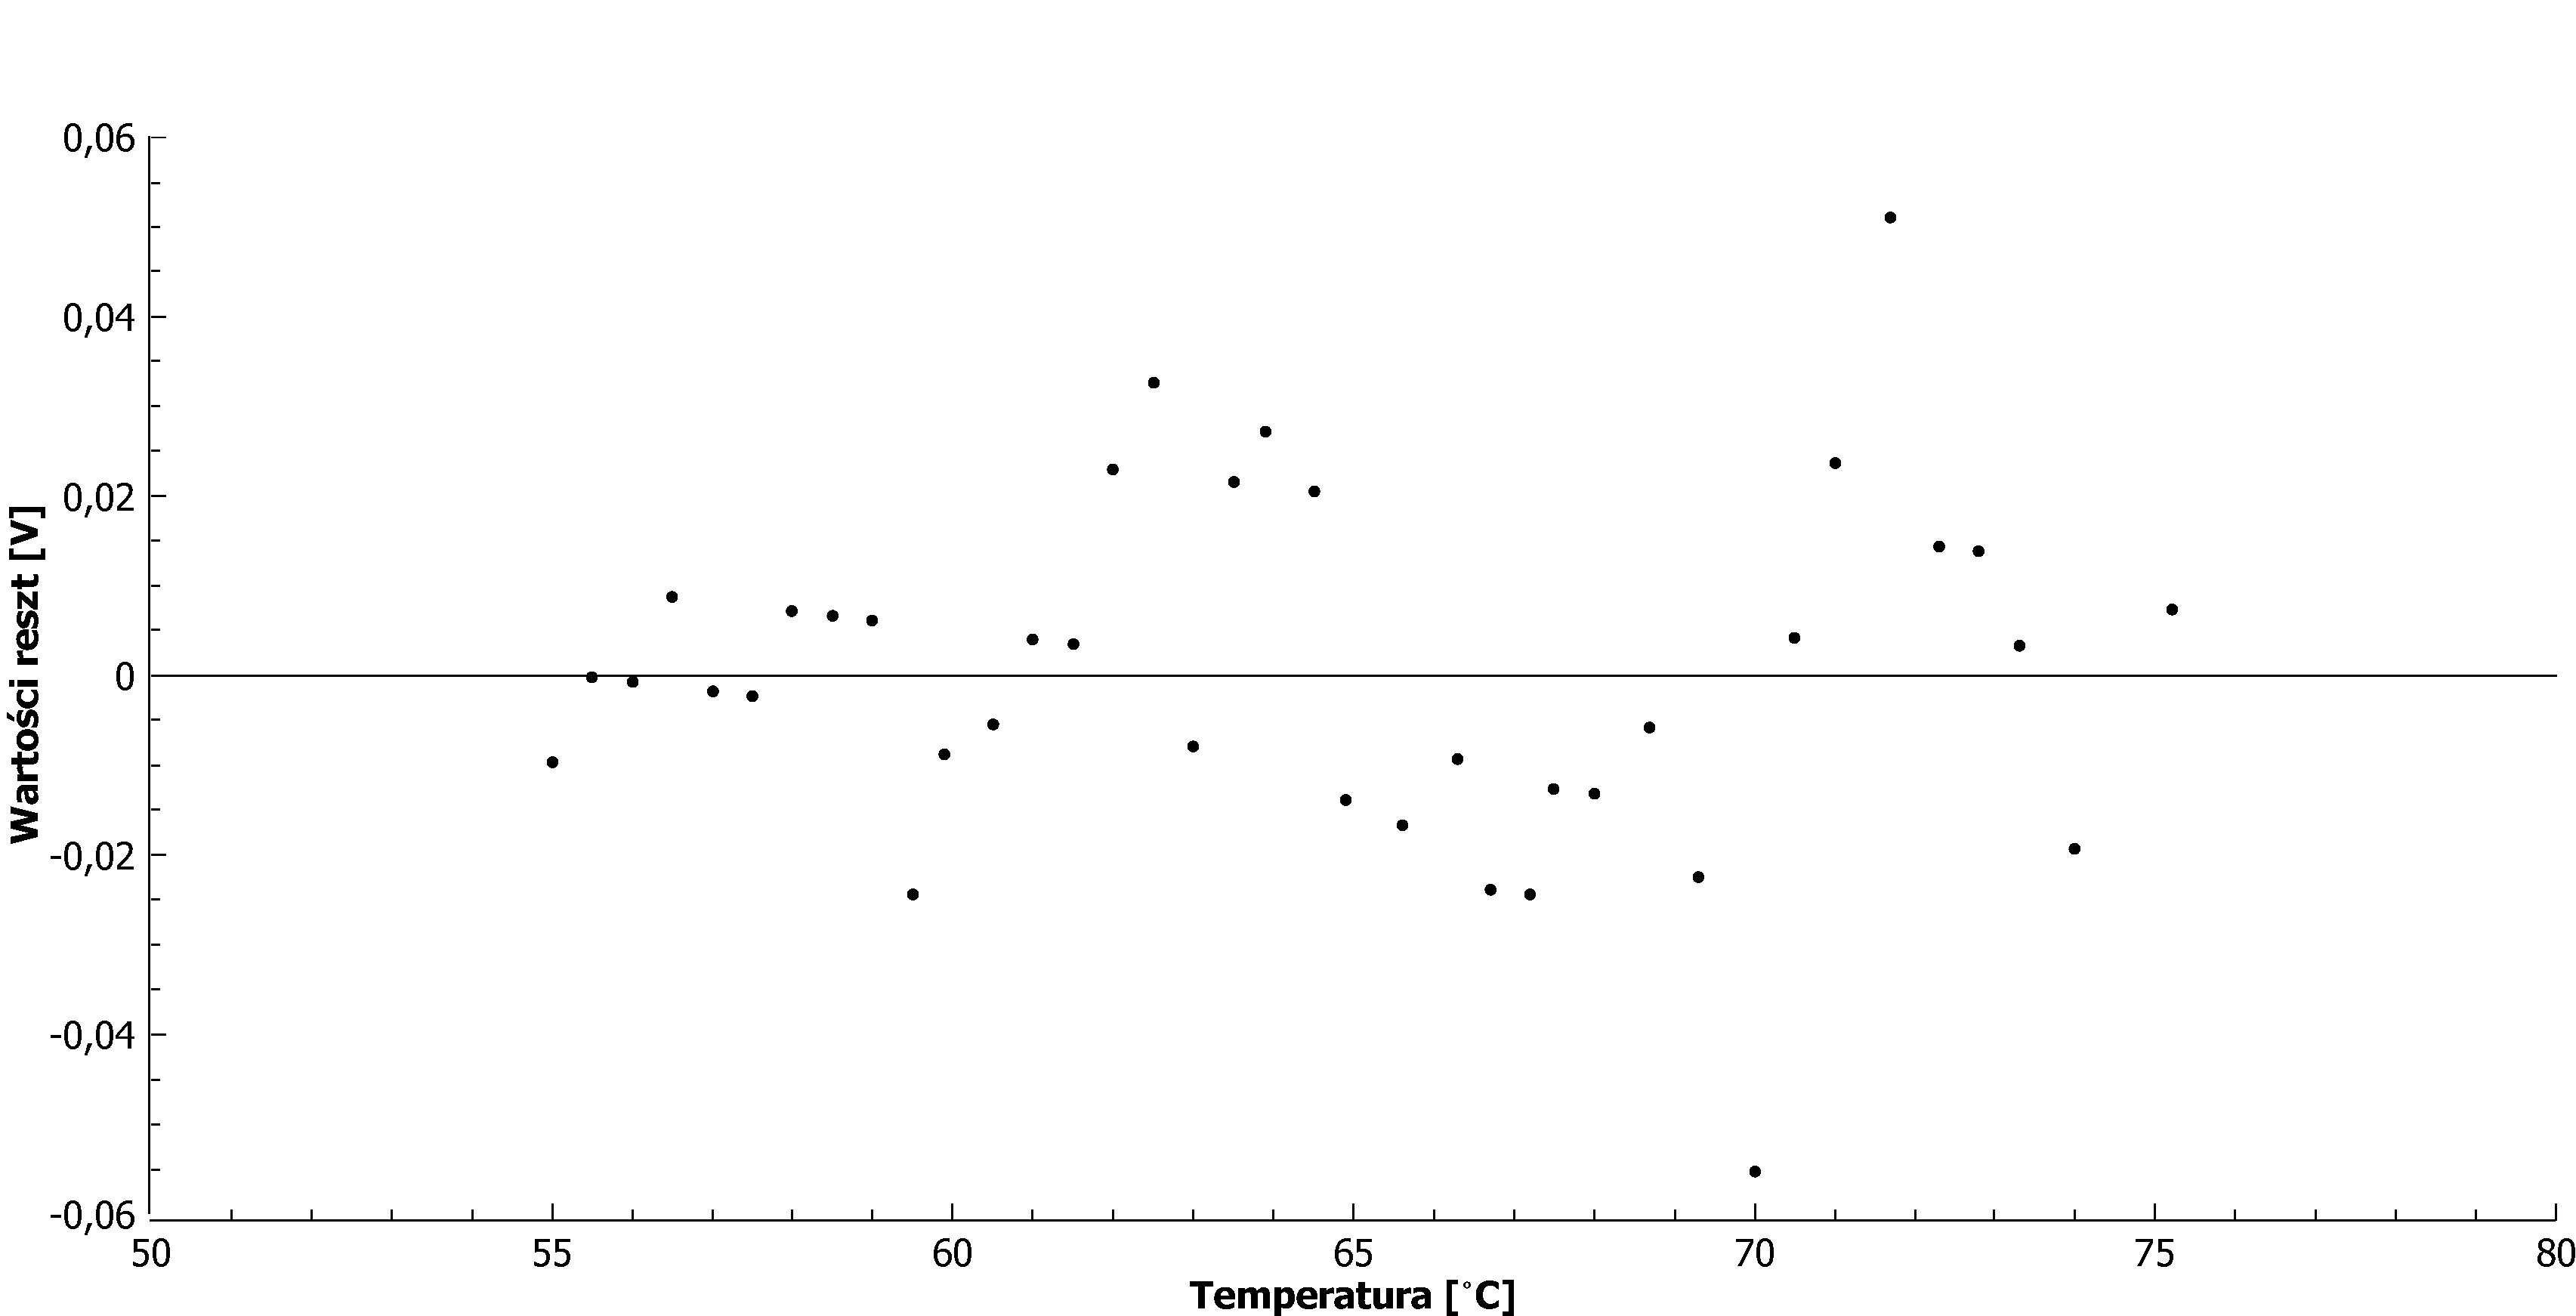
\includegraphics[width=12cm]{rys5.pdf} 
\centering
\caption{Wykres reszt $\epsilon_{i}$ [V]}
\end{figure}
Jak widać reszty są w miarę równomiernie rozłożone po obu stronach osi $x=0$. Jednak można zauważyć coś na kształt zależności sinusoidalnej. Być może jest to przypadek albo w trakcie pomiarów doszło do wprowadzenia błędu systematycznego. Jednak na potrzeby dalszej analizy danych założono, iż nie ma żadnych błędów systematycznych. 

Ostatnim krokiem pozostałym do stworzenia termometru jest odwrócenie zależności wyrażonej przez Równanie (4) oraz wyznaczenie niepewności otrzymanej w ten sposób wartości temperatury. Zależność $t(U)$ można zapisać w sposób:
\begin{equation}
t(U)=HU+G,
\end{equation}
gdzie $H=1/h=-7,19597$ $^{\circ}$C/V  oraz $G=-g/h=140,41393$ $^{\circ}$C. Niepewności tych współczynników można wyznaczyć korzystając z Równania (10).
Otrzymano w ten sposób:
\begin{eqnarray}
u_{H}=\dfrac{u_{h}}{h^2}, \\
u_{G}=\sqrt{\dfrac{u_{g}^2}{h^2}+\dfrac{u_{h}^2 g^2}{h^4}-2\dfrac{g}{h^3}c_{gh}}.
\end{eqnarray}
Wartości tych niepewności wynoszą: $u_{H}=0,06900$ $^{\circ}$C/V, $u_{G}=0,72488$ $^{\circ}$C. 
Ostatecznie można zapisać: $\bar{h}=-7,196\pm0,069$ $^{\circ}$C/V oraz $\bar{G}=140,41\pm0,72$ $^{\circ}$C.
Dodatkowo można wyznaczyć ocenę kowariancji $G$ i $H$ korzystając z Równania (14), który po dostosowaniu do nowych zmiennych daje następujący wynik:
\begin{equation}
c_{HG}=\dfrac{-g}{h^4}u_{h}^2+\dfrac{c_{hg}}{h^3}.
\end{equation}
Po podstawieniu danych liczbowych otrzymano $c_{HG}=-0,04987$ $^{\circ}$C$^2$/V oraz $\rho_{HG}=-0,99706$. W tym przypadku $\rho_{HG}\neq\rho_{hg}$ ponieważ wartości pochodnej niepewności i kowariancji nie redukują się wzajemnie. Przy takim zestawie danych można wyznaczyć niepewność temperatury $t$ dla danego napięcia $U$ stosując Równanie (10) do Równania (15). Otrzymano:
\begin{equation}
u_{t}=\sqrt{H^2u_{U}^2+U^2u_{H}^2+u_{G}^2+2U^2c_{HG}}
\end{equation}
Niepewność napięcia $u_{U}$ można, dla miernika Brymen, obliczyć z Równania (8). W ten sposób otrzymujemy kompletną informację o wartości temperatury i jej niepewności. Dla przykładu można założyć, iż zmierzono napięcie o wartości $U=7,82$ V. W takim wypadku wartość temperatury wraz z niepewnością powinna wynosić $t=84,14\pm0,35$ $^{\circ}$C. Jak widać niepewność ta jest wysoka, w szczególności porównując ją do działki odczytu termometru wzorcowego otrzymujemy trzykrotny wzrost niepewności. 

Aby dopełnić analizę danych należałoby wykonać wykres reszt $\delta_{i}=t_{i}-(HU_{i}+G)$. Wartości reszt przedstawiono w Tabeli 7. Na podstawie tych danych stworzono wykres przedstawiony na Rysunku 6.

\begin{center}
 \begin{table}[h!]
 \centering
 \caption{Wartości reszt}
 \begin{tabular}{|c|c|c|c|c|c|c|c|c|c|c|c|c|c|c|c|c|c|c|c|c|c|}
\hline
Temperatura t [$^{\circ}$C]&75,2     & 74       & 73,3     & 72,8     & 72,3     & 71,7     & 71       \\ \hline
Reszta [$^{\circ}$C]&0,05350  & -0,13906 & 0,02445  & 0,10013  & 0,10385  & 0,36736  & 0,17108  \\ \hline
Temperatura t [$^{\circ}$C]&70,5     & 70       & 69,3     & 68,7     & 68       & 67,5     & 67,2     \\ \hline
Reszta [$^{\circ}$C]&0,03088  & -0,39716 & -0,16169 & -0,04209 & -0,09445 & -0,09073 & -0,17486 \\ \hline
Temperatura t [$^{\circ}$C]&66,7     & 66,3     & 65,6     & 64,9     & 64,5     & 63,9     & 63,5     \\ \hline
Reszta [$^{\circ}$C]&-0,17114 & -0,06742 & -0,11978 & -0,10019 & 0,14745  & 0,19509  & 0,15489  \\ \hline
Temperatura t [$^{\circ}$C]&63       & 62,5     & 62       & 61,5     & 61       & 60,5     & 59,9     \\ \hline
Reszta [$^{\circ}$C]&-0,05727 & 0,23428  & 0,16604  & 0,02584  & 0,02956  & -0,03869 & -0,06301 \\ \hline
Temperatura t [$^{\circ}$C]&59,5     & 59       & 58,5     & 58       & 57,5     & 57       & 56,5     \\ \hline
Reszta [$^{\circ}$C]&-0,17517 & 0,04443  & 0,04814  & 0,05186  & -0,01638 & -0,01266 & 0,06302  \\ \hline
Temperatura t [$^{\circ}$C]&56       &          &          & 55,5     &          &          & 55       \\ \hline
Reszta [$^{\circ}$C]&-0,00523 &          &          & -0,00151 &          &          & -0,06975 \\ \hline
\end{tabular}
 \end{table}
 \end{center}


\begin{figure}[h!]
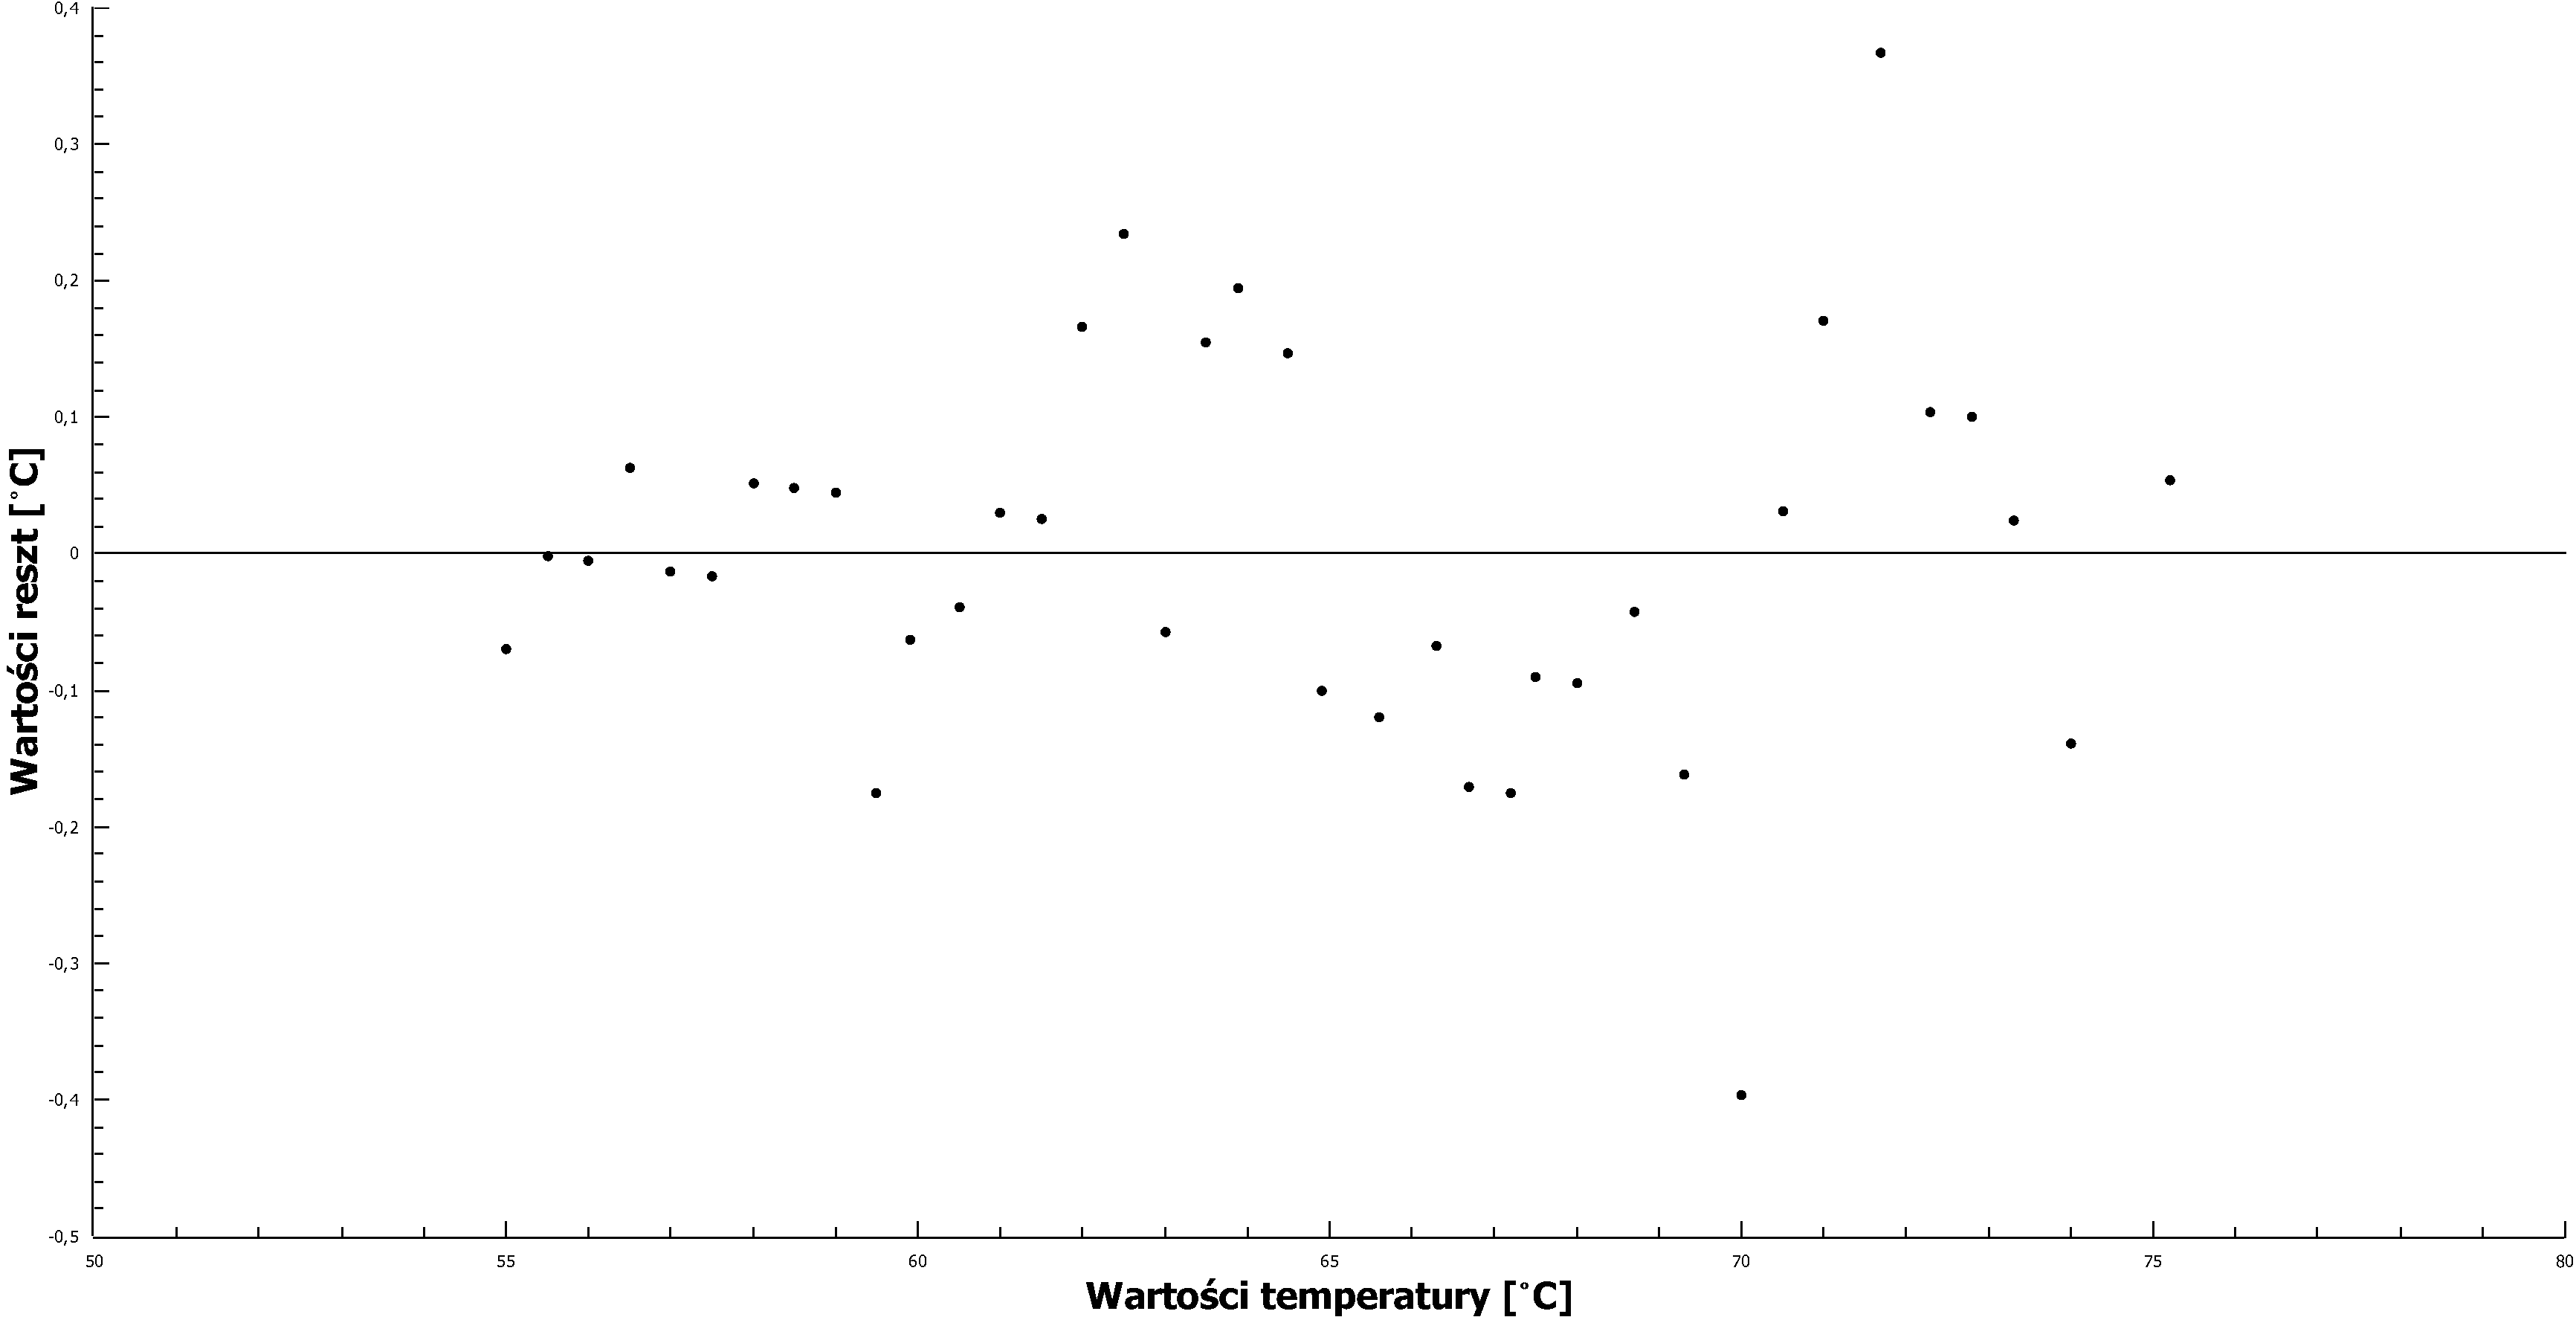
\includegraphics[width=12cm]{rys6.pdf} 
\centering
\caption{Wykres reszt $\delta_{i}$ [$^{\circ}$C]}
\end{figure}

Wykres ten przyjmuje identyczny kształt jak wykres reszt $\epsilon_{i}$, jednak w tym przypadku zmieniła się skala. Dodatkowo wykres ten pozwala określić, w jakim przedziale temperatury pomiary termistorem byłyby najdokładniejsze. Jak widać najmniejsze odchylenie przypada na przedział poniżej 60 $^{\circ}$C. Różnica pomiędzy wartościami teoretycznymi, a eksperymentalnymi rośnie gwałtownie powyżej tej granicy. W tym przedziale termistor staje się niedokładnym termometrem, jednak dla wartości poniżej tej wartości termistor wykazuje się zadowalającą dokładnością.

\begin{center}
\textbf{\subsection*{DYSKUSJA WYNIKÓW I WNIOSKI}}
\end{center}  
Otrzymana wartość niepewności dla przykładowego napięcia, jak i struktura wykresu reszt przedstawiona na Rysunku 6 pozwala stwierdzić, iż termometr oparty o ten termistor byłby wysoce niedokładny. Może to wynikać z faktu błędnego wybrania opornika do dzielnika napięć. Jednak w tym przypadku wybór był niewielki, więc możliwość ponownej kalibracji przyrządu przy oporniki o oporze bliższym wartości oporu teoretycznego pozwoliłaby rozwiązać tę kwestię. Dodatkowo można sądzić, iż w pomiarach miał miejsce błąd systematyczny. Tłumaczyłoby to błędną kalibrację przyrządu, jak i otrzymanie skrajnych współczynników w porównaniu z innymi termistorami. Jeśli błąd systematyczny faktycznie miał miejsce, to miał on swoje źródło w mierniku. Wykorzystanie innego miernika pozwoliłoby na lepszą ocenę sytuacji.


\begin{center}
\begin{thebibliography}{9}

\bibitem{pf}
 H. Szydłowski,
  \emph{Pracownia fizyczna},
  PWN, Warszawa, 1973, s. 385.
  
  \bibitem{b1}
  Praca zbiorowa,
  \emph{Multimetry cyfrowe BM805, BM806T, BM807},
  BRYMEN Technology Co., Taiwan, s. 20.

  \bibitem{tay1}
 J. R. Taylor,
 \emph{Wstęp do analizy błędu pomiarowego},
 PWN, Warszawa, 1995, s. 175.
 
 
  \bibitem{tay2}
 J. R. Taylor,
 \emph{Wstęp do analizy błędu pomiarowego},
 PWN, Warszawa, 1995, s. 197.
 
  \end{thebibliography}



\begin{center}
\textbf{\subsection*{DODATEK}}
\end{center} 



\begin{center}
 \begin{table}[h!]
 \centering
 \caption{Wartości oporu oraz jego niepewności}
 \label{t1}
 \begin{tabular}{|c|c|c|c|c|c|c|c|c|c|c|c|c|c|c|c|c|c|c|c|c|c|}
 \hline
Opór $r$ [k$\Omega$]&Wartość w& Wartość nc&Wartość $\Delta_{p}$ [k$\Omega$]& $u_{i}$ [k$\Omega$]\\ 
\hline
40,3 & 0,006 & 0,4 & 0,64180 & 0,37054 \\ \hline
41,2 & 0,006 & 0,4 & 0,64720 & 0,37366 \\ \hline
42,1 & 0,006 & 0,4 & 0,65260 & 0,37678 \\ \hline
43,3 & 0,006 & 0,4 & 0,65980 & 0,38094 \\ \hline
44   & 0,006 & 0,4 & 0,66400 & 0,38336 \\ \hline
45   & 0,006 & 0,4 & 0,67000 & 0,38682 \\ \hline
45,5 & 0,006 & 0,4 & 0,67300 & 0,38856 \\ \hline
47,2 & 0,006 & 0,4 & 0,68320 & 0,39445 \\ \hline
48   & 0,006 & 0,4 & 0,68800 & 0,39722 \\ \hline
49,6 & 0,006 & 0,4 & 0,69760 & 0,40276 \\ \hline
50,8 & 0,006 & 0,4 & 0,70480 & 0,40692 \\ \hline
52,2 & 0,006 & 0,4 & 0,71320 & 0,41177 \\ \hline
53,7 & 0,006 & 0,4 & 0,72220 & 0,41696 \\ \hline
55,1 & 0,006 & 0,4 & 0,73060 & 0,42181 \\ \hline
55,6 & 0,006 & 0,4 & 0,73360 & 0,42354 \\ \hline
58,4 & 0,006 & 0,4 & 0,75040 & 0,43324 \\ \hline
59,3 & 0,006 & 0,4 & 0,75580 & 0,43636 \\ \hline
60,2 & 0,006 & 0,4 & 0,76120 & 0,43948 \\ \hline
61,8 & 0,006 & 0,4 & 0,77080 & 0,44502 \\ \hline
62,2 & 0,006 & 0,4 & 0,77320 & 0,44641 \\ \hline
63,1 & 0,006 & 0,4 & 0,77860 & 0,44952 \\ \hline
64   & 0,006 & 0,4 & 0,78400 & 0,45264 \\ \hline
65   & 0,006 & 0,4 & 0,79000 & 0,45611 \\ \hline
65,9 & 0,006 & 0,4 & 0,79540 & 0,45922 \\ \hline
66,6 & 0,006 & 0,4 & 0,79960 & 0,46165 \\ \hline
67,6 & 0,006 & 0,4 & 0,80560 & 0,46511 \\ \hline
69   & 0,006 & 0,4 & 0,81400 & 0,46996 \\ \hline
70   & 0,006 & 0,4 & 0,82000 & 0,47343 \\ \hline
70,7 & 0,006 & 0,4 & 0,82420 & 0,47585 \\ \hline
71,2 & 0,006 & 0,4 & 0,82720 & 0,47758 \\ \hline
73   & 0,006 & 0,4 & 0,83800 & 0,48382 \\ \hline

 \end{tabular}
 \end{table}
 \end{center}




\begin{center}
 \begin{table}[h!]
 \centering
 \caption{Wartości oporu oraz jego niepewności}
 \label{t2}
 \begin{tabular}{|c|c|c|c|c|c|c|c|c|c|c|c|c|c|c|c|c|c|c|c|c|c|}
 \hline
Opór $r$ [k$\Omega$]&Wartość w& Wartość nc&Wartość $\Delta_{p}$ [k$\Omega$]& $u_{i}$ [k$\Omega$]\\ 
\hline
74,3 & 0,006 & 0,4 & 0,84580 & 0,48832 \\ \hline
75,7 & 0,006 & 0,4 & 0,85420 & 0,49317 \\ \hline
76,8 & 0,006 & 0,4 & 0,86080 & 0,49698 \\ \hline
78,2 & 0,006 & 0,4 & 0,86920 & 0,50183 \\ \hline
79,8 & 0,006 & 0,4 & 0,87880 & 0,50738 \\ \hline
81   & 0,006 & 0,4 & 0,88600 & 0,51153 \\ \hline
82,4 & 0,006 & 0,4 & 0,89440 & 0,51638 \\ \hline
83,8 & 0,006 & 0,4 & 0,90280 & 0,52123 \\ \hline
85   & 0,006 & 0,4 & 0,91000 & 0,52539 \\ \hline
86,2 & 0,006 & 0,4 & 0,91720 & 0,52955 \\ \hline
87,6 & 0,006 & 0,4 & 0,92560 & 0,53440 \\ \hline
89,1 & 0,006 & 0,4 & 0,93460 & 0,53959 \\ \hline
91   & 0,006 & 0,4 & 0,94600 & 0,54617 \\ \hline
92,5 & 0,006 & 0,4 & 0,95500 & 0,55137 \\ \hline
94,1 & 0,006 & 0,4 & 0,96460 & 0,55691 \\ \hline
95,9 & 0,006 & 0,4 & 0,97540 & 0,56315 \\ \hline
551  & 0,01  & 4   & 9,51000 & 5,49060 \\ \hline
543  & 0,01  & 4   & 9,43000 & 5,44441 \\ \hline
537  & 0,01  & 4   & 9,37000 & 5,40977 \\ \hline
524  & 0,01  & 4   & 9,24000 & 5,33472 \\ \hline
509  & 0,01  & 4   & 9,09000 & 5,24811 \\ \hline
495  & 0,01  & 4   & 8,95000 & 5,16728 \\ \hline
484  & 0,01  & 4   & 8,84000 & 5,10378 \\ \hline
474  & 0,01  & 4   & 8,74000 & 5,04604 \\ \hline
459  & 0,01  & 4   & 8,59000 & 4,95944 \\ \hline
441  & 0,01  & 4   & 8,41000 & 4,85552 \\ \hline
434  & 0,01  & 4   & 8,34000 & 4,81510 \\ \hline
425  & 0,01  & 4   & 8,25000 & 4,76314 \\ \hline
420  & 0,01  & 4   & 8,20000 & 4,73427 \\ \hline
413  & 0,01  & 4   & 8,13000 & 4,69386 \\ \hline
410  & 0,01  & 4   & 8,10000 & 4,67654 \\ \hline
400  & 0,01  & 4   & 8,00000 & 4,61880 \\ \hline
 \end{tabular}
 \end{table}
 \end{center}
 
\begin{center}
 \begin{table}[h!]
 \centering
 \caption{Wartości oporu oraz jego niepewności}
 \label{t3}
 \begin{tabular}{|c|c|c|c|c|c|c|c|c|c|c|c|c|c|c|c|c|c|c|c|c|c|}
\hline 
 x [1/K] & $\eta$ & $u_{\eta i}$ & $1/u_{\eta i}$       & $S_{i}$\\ \hline
0,00286  & 3,69635   & 0,00919 & 108,75919 & 11828,56121              \\ \hline
0,00287  & 3,71844   & 0,00907 & 110,26034 & 12157,34299              \\ \hline
0,00287  & 3,74005   & 0,00895 & 111,73665 & 12485,07937              \\ \hline
0,00288  & 3,76815   & 0,00880 & 113,66747 & 12920,29486              \\ \hline
0,00288  & 3,78419   & 0,00871 & 114,77445 & 13173,17463              \\ \hline
0,00289  & 3,80666   & 0,00860 & 116,33177 & 13533,08086              \\ \hline
0,00289  & 3,81771   & 0,00854 & 117,10002 & 13712,41409              \\ \hline
0,00290  & 3,85439   & 0,00836 & 119,66159 & 14318,89606              \\ \hline
0,00291  & 3,87120   & 0,00828 & 120,84075 & 14602,48783              \\ \hline
0,00291  & 3,90399   & 0,00812 & 123,15040 & 15166,02138              \\ \hline
0,00292  & 3,92790   & 0,00801 & 124,84135 & 15585,36180              \\ \hline
0,00293  & 3,95508   & 0,00789 & 126,77096 & 16070,87754              \\ \hline
0,00294  & 3,98341   & 0,00776 & 128,78860 & 16586,50401              \\ \hline
0,00294  & 4,00915   & 0,00766 & 130,62688 & 17063,38213              \\ \hline
0,00295  & 4,01818   & 0,00762 & 131,27321 & 17232,65496              \\ \hline
0,00296  & 4,06732   & 0,00742 & 134,79713 & 18170,26655              \\ \hline
0,00296  & 4,08261   & 0,00736 & 135,89655 & 18467,87245              \\ \hline
0,00297  & 4,09767   & 0,00730 & 136,98037 & 18763,62212              \\ \hline
0,00297  & 4,12390   & 0,00720 & 138,86967 & 19284,78462              \\ \hline
0,00298  & 4,13035   & 0,00718 & 139,33466 & 19414,14788              \\ \hline
0,00298  & 4,14472   & 0,00712 & 140,37042 & 19703,85371              \\ \hline
0,00298  & 4,15888   & 0,00707 & 141,39190 & 19991,67014              \\ \hline
0,00299  & 4,17439   & 0,00702 & 142,51051 & 20309,24531              \\ \hline
0,00299  & 4,18814   & 0,00697 & 143,50283 & 20593,06122              \\ \hline
0,00300  & 4,19870   & 0,00693 & 144,26536 & 20812,49479              \\ \hline
0,00300  & 4,21361   & 0,00688 & 145,34091 & 21123,97922              \\ \hline
0,00301  & 4,23411   & 0,00681 & 146,82003 & 21556,12168              \\ \hline
0,00301  & 4,24850   & 0,00676 & 147,85800 & 21861,98691              \\ \hline
0,00301  & 4,25845   & 0,00673 & 148,57558 & 22074,70263              \\ \hline
0,00302  & 4,26549   & 0,00671 & 149,08368 & 22225,94271              \\ \hline
0,00302  & 4,29046   & 0,00663 & 150,88271 & 22765,59145              \\ \hline
0,00302  & 4,30811   & 0,00657 & 152,15343 & 23150,66767              \\ \hline
 0,00303  & 4,32678   & 0,00651 & 153,49596 & 23561,00869              \\ \hline
0,00303  & 4,34120   & 0,00647 & 154,53241 & 23880,26699              \\ \hline
0,00304  & 4,35927   & 0,00642 & 155,82878 & 24282,60781              \\ \hline
0,00304  & 4,37952   & 0,00636 & 157,27999 & 24736,99498              \\ \hline
0,00305  & 4,39445   & 0,00632 & 158,34776 & 25074,01312              \\ \hline
0,00305  & 4,41159   & 0,00627 & 159,57176 & 25463,14816              \\ \hline
0,00306  & 4,42843   & 0,00622 & 160,77299 & 25847,95513              \\ \hline
0,00306  & 4,44265   & 0,00618 & 161,78497 & 26174,37508              \\ \hline
0,00307  & 4,45667   & 0,00614 & 162,78105 & 26497,67044              \\ \hline
0,00307  & 4,47278   & 0,00610 & 163,92356 & 26870,93480              \\ \hline
0,00308  & 4,48976   & 0,00606 & 165,12490 & 27266,23098              \\ \hline
\end{tabular}
 \end{table}
 \end{center}
 
 \begin{center}
 \begin{table}[h!]
 \centering
 \caption{Wartości oporu oraz jego niepewności}
 \label{t4}
 \begin{tabular}{|c|c|c|c|c|c|c|c|c|c|c|c|c|c|c|c|c|c|c|c|c|c|}
 \hline
 x [1/K] & $\eta$ & $u_{\eta i}$ & $1/u_{\eta i}$       & $S_{i}$\\ \hline
0,00308  & 4,51086   & 0,00600 & 166,61377 & 27760,14732              \\ \hline
0,00309  & 4,52721   & 0,00596 & 167,76408 & 28144,78770              \\ \hline
0,00309  & 4,54436   & 0,00592 & 168,96743 & 28549,99171              \\ \hline
0,00310  & 4,56331   & 0,00587 & 170,29288 & 28999,66403              \\ \hline
0,00360  & 6,31173   & 0,00996 & 100,35331 & 10070,78718              \\ \hline
0,00359  & 6,29711   & 0,01003 & 99,73527  & 9947,12392               \\ \hline
0,00359  & 6,28600   & 0,01007 & 99,26481  & 9853,50280               \\ \hline
0,00358  & 6,26149   & 0,01018 & 98,22453  & 9648,05757               \\ \hline
0,00358  & 6,23245   & 0,01031 & 96,98722  & 9406,52151               \\ \hline
0,00357  & 6,20456   & 0,01044 & 95,79499  & 9176,67988               \\ \hline
0,00356  & 6,18208   & 0,01054 & 94,83174  & 8993,05911               \\ \hline
0,00356  & 6,16121   & 0,01065 & 93,93502  & 8823,78815               \\ \hline
0,00355  & 6,12905   & 0,01080 & 92,55079  & 8565,64947               \\ \hline
0,00354  & 6,08904   & 0,01101 & 90,82454  & 8249,09760               \\ \hline
0,00353  & 6,07304   & 0,01109 & 90,13310  & 8123,97564               \\ \hline
0,00353  & 6,05209   & 0,01121 & 89,22686  & 7961,43251               \\ \hline
0,00352  & 6,04025   & 0,01127 & 88,71480  & 7870,31529               \\ \hline
0,00352  & 6,02345   & 0,01137 & 87,98733  & 7741,77004               \\ \hline
0,00351  & 6,01616   & 0,01141 & 87,67171  & 7686,32830               \\ \hline
0,00351  & 5,99146   & 0,01155 & 86,60254  & 7500,00000               \\ \hline
 \end{tabular}
 \end{table}
 \end{center}
 
 
 \begin{center}
 \begin{table}[h!]
 \centering
 \caption{Wartości oporu oraz jego niepewności}
 \label{t5}
 \begin{tabular}{|c|c|c|c|c|c|c|c|c|c|c|c|c|c|c|c|c|c|c|c|c|c|}
 \hline
$S_{xi}$ [1/K]& $S_{\eta i}$ & $S_{tti}$ [1/K$^2$]&$S_{\eta ti}$ [1/K] \\ \hline
33,78624                    & 43722,51959                   & 0,09650         & 124,88580                   \\ \hline
34,84478                    & 45206,32928                   & 0,09987                           & 129,56816                   \\ \hline
35,86636                    & 46694,79288                   & 0,10303        & 134,14189                   \\ \hline
37,17001                    & 48685,64312                   & 0,10693      & 140,06226                   \\ \hline
37,95210                    & 49849,79087                   & 0,10934              & 143,61795                   \\ \hline
39,07907                    & 51515,87130                   & 0,11285              & 148,76082                   \\ \hline
39,63125                    & 52350,05228                   & 0,11454                & 151,30073                   \\ \hline
41,55222                    & 55190,66553                   & 0,12058              & 160,15863                   \\ \hline
42,46144                    & 56529,16565                   & 0,12347                    & 164,37675                   \\ \hline
44,20292                    & 59208,00845                   & 0,12883                      & 172,56779                   \\ \hline
45,53129                    & 61217,68580                   & 0,13302                         & 178,84220                   \\ \hline
47,07346                    & 63561,64643                   & 0,13788                                      & 186,17940                   \\ \hline
48,71220                    & 66070,89571                   & 0,14306                                      & 194,04081                   \\ \hline
50,21596                    & 68409,65360                   & 0,14778                                      & 201,32329                   \\ \hline
50,78884                    & 69243,96469                   & 0,14969                                      & 204,07888                   \\ \hline
53,74228                    & 73904,21385                   & 0,15895                                      & 218,58685                   \\ \hline
54,70341                    & 75397,10791                   & 0,16204                                      & 223,33267                   \\ \hline
55,66189                    & 76887,17557                   & 0,16512                                      & 228,08418                   \\ \hline
57,34399                    & 79528,58819                   & 0,17051                                      & 236,48108                   \\ \hline
57,76301                    & 80187,32276                   & 0,17186                                      & 238,58174                   \\ \hline
58,71232                    & 81666,97171                   & 0,17495                                      & 243,34616                   \\ \hline
59,65882                    & 83143,01874                   & 0,17803                                      & 248,11405                   \\ \hline
60,69709                    & 84778,65510                   & 0,18140                                      & 253,37315                   \\ \hline
61,63742                    & 86246,59133                   & 0,18449                                      & 258,14604                   \\ \hline
 \end{tabular}
 \end{table}
 \end{center}


\begin{center}
 \begin{table}[h!]
 \centering
 \caption{Wartości oporu oraz jego niepewności}
 \label{t6}
 \begin{tabular}{|c|c|c|c|c|c|c|c|c|c|c|c|c|c|c|c|c|c|c|c|c|c|}
 \hline
 $S_{xi}$ [1/K]& $S_{\eta i}$ & $S_{tti}$ [1/K$^2$]&$S_{\eta ti}$ [1/K]\\
 \hline
62,38757                    & 87385,51715                   & 0,18701                                      & 261,94699                   \\ \hline
63,41633                    & 89008,16746                   & 0,19038                                      & 267,21155                   \\ \hline
64,81095                    & 91270,91501                   & 0,19486                                      & 274,41646                   \\ \hline
65,80971                    & 92880,54738                   & 0,19810                                      & 279,59226                   \\ \hline
66,49007                    & 94003,91970                   & 0,20027                                      & 283,14434                   \\ \hline
67,02637                    & 94804,59900                   & 0,20213                                      & 285,90048                   \\ \hline
68,75745                    & 97674,84676                   & 0,20766                                      & 295,00105                   \\ \hline
70,02622                    & 99735,64492                   & 0,21182                                      & 301,68072                   \\ \hline
71,37537                    & 101943,25786                  & 0,21622                                      & 308,82538                   \\ \hline
72,45227                    & 103669,12589                  & 0,21982                                      & 314,53011                   \\ \hline
73,78489                    & 105854,43518                  & 0,22420                                      & 321,64824                   \\ \hline
75,27996                    & 108336,25094                  & 0,22909                                      & 329,69036                   \\ \hline
76,42186                    & 110186,47574                  & 0,23292                                      & 335,83199                   \\ \hline
77,72634                    & 112332,85360                  & 0,23726                                      & 342,89638                   \\ \hline
79,02157                    & 114465,93769                  & 0,24158                                      & 349,94172                   \\ \hline
80,14199                    & 116283,62032                  & 0,24538                                      & 356,04293                   \\ \hline
81,25627                    & 118091,37761                  & 0,24918                                      & 362,13241                   \\ \hline
82,52744                    & 120187,80657                  & 0,25346                                      & 369,12717                   \\ \hline
83,87029                    & 122418,81506                  & 0,25798                                      & 376,55741                   \\ \hline
85,52109                    & 125222,12445                  & 0,26347                                      & 385,77364                   \\ \hline
86,83983                    & 127417,32616                  & 0,26794                                      & 393,14201                   \\ \hline
88,22618                    & 129741,38454                  & 0,27264                                      & 400,93135                   \\ \hline
89,75445                    & 132334,34036                  & 0,27779                                      & 409,57704                   \\ \hline
36,21283                    & 63564,13802                   & 0,13022                                      & 228,56576                   \\ \hline
35,74245                    & 62638,12675                   & 0,12843                                      & 225,07412                   \\ \hline
35,36792                    & 61939,09983                   & 0,12695                                      & 222,32268                   \\ \hline
34,56846                    & 60411,23225                   & 0,12386                                      & 216,45013                   \\ \hline
33,64278                    & 58625,65633                   & 0,12032                                      & 209,67688                   \\ \hline
32,75046                    & 56937,24038                   & 0,11688                                      & 203,20214                   \\ \hline
32,03797                    & 55595,85499                   & 0,11414                                      & 198,06147                   \\ \hline
31,37905                    & 54365,18818                   & 0,11159                                      & 193,33282                   \\ \hline
30,38542                    & 52499,29571                   & 0,10779                                      & 186,23376                   \\ \hline
29,20035                    & 50229,12547                   & 0,10336                                      & 177,80221                   \\ \hline
28,70663                    & 49337,26585                   & 0,10144                                      & 174,33663                   \\ \hline
28,10248                    & 48183,29944                   & 0,09920                                      & 170,07871                   \\ \hline
27,73191                    & 47538,70900                   & 0,09772                                      & 167,50778                   \\ \hline
27,24057                    & 46632,14610                   & 0,09585                                      & 164,08215                   \\ \hline
27,01697                    & 46242,15906                   & 0,09496                                      & 162,53834                   \\ \hline
26,31579                    & 44935,98410                   & 0,09234                                      & 157,67012                   \\ \hline
 \end{tabular}
 \end{table}
 \end{center}
 
\end{center}
\end{document}